% ============================================================================
%  Cell-state reachability: a convex-cone oracle for feasibility verdicts
%  ICML 2026 format (preprint mode) --- compiled with tectonic / pdflatex
% ============================================================================
\documentclass{article}

% ---- Encoding: accented author names in the bibliography (Barabási, Zañudo, ...) ----
\usepackage[T1]{fontenc}
\usepackage[utf8]{inputenc}

% ---- Recommended figure / typesetting packages ----
\usepackage{microtype}
\usepackage{graphicx}
\graphicspath{{figures/}}
\usepackage{subcaption}
\usepackage{booktabs}

% ---- hyperref (loaded before icml2026 as in the ICML template) ----
\usepackage{hyperref}
\newcommand{\theHalgorithm}{\arabic{algorithm}}

% ---- ICML 2026 style: preprint mode (shows authors, honest "Preprint" footer) ----
\usepackage[preprint]{icml2026}

% ---- Math ----
\usepackage{amsmath}
\usepackage{amssymb}
\usepackage{mathtools}
\usepackage{amsthm}
\usepackage{bm}

% ---- Convenience macros ----
\newcommand{\reach}{\textsc{Reach}}
\newcommand{\cone}{\mathcal{C}}
\newcommand{\Emat}{\mathbf{E}}
\newcommand{\dvec}{\mathbf{d}}
\newcommand{\wvec}{\mathbf{w}}
\newcommand{\Rnn}{\mathbb{R}_{\geq 0}}

% ---- Title (a short running form is required for the page header) ----
\icmltitlerunning{Can knockdown point a cell toward the target state?}

\begin{document}

\twocolumn[
\icmltitle{Can Knockdown Point a Cell Toward the Target State?\\
A Convex-Cone Feasibility Test with Dual Certificates\\
from Measured Genome-Scale Perturbation Screens}

\begin{icmlauthorlist}
\icmlauthor{Cell-State Reachability Project}{bwc}
\end{icmlauthorlist}

\icmlaffiliation{bwc}{Built with Claude --- Life Sciences (Research Track)}

\icmlcorrespondingauthor{Cell-State Reachability Project}%
{github.com/MasalaKimchi/cell-state-reachability}

\icmlkeywords{cell-state engineering, convex cone, non-negative least squares,
Perturb-seq, feasibility verdict, CRISPRi, reachability}

\vskip 0.3in
]

% must follow the closing ] of \twocolumn[ ...
\printAffiliationsAndNotice{}

\begin{abstract}
Combinatorial perturbation screens explode super-linearly: 100 single perturbations imply
roughly 5{,}000 pairs and 160{,}000 triples, and only a fraction of combinations produce
cell states that the single perturbations cannot already reach in combination. We ask two
questions a screening team faces directly---which unmeasured combinations are worth running,
and which measured ones are genuinely \emph{emergent} rather than additive noise---and answer
both from measured effects alone, with a certificate rather than a prediction. We treat a
screen's single-gene effect vectors as a fixed dictionary and define a combination as emergent
when its measured effect leaves the non-negative cone of the single effects. Non-negative
least squares decides cone membership exactly; on the outside, convex duality (a Farkas/KKT
separator) certifies the unreachable direction. On the Norman 2019 CRISPRa combinatorial
screen (data file labelled A549; the canonical line for this study is K562), all $131$ measured
doubles are geometrically outside the single-gene cone, but the raw unreachable fraction is
confounded by effect magnitude (Spearman $-0.56$; only a minority of doubles clear their own
split-half noise floor). A noise-injection null removes the confound and certifies $129/131$
emergent at $p<0.05$, of which $35$ also clear a $1.9\times$ floor; the certificate recovers
classical synergy (partial Spearman $0.62$ controlling for magnitude). A training-free triage
score---the negative cosine between two single effects---ranks emergent combinations $2.4\times$
above base rate (raw label; $1.4\times$ on the noise-robust label) \emph{without measuring the
combination}. A self-contained learned neural baseline ties the trivial additive baseline for
blind prediction (held-out cosine $0.896$ vs.\ $0.897$), reproducing the 2025--2026 finding
that learned models do not beat additivity out-of-sample; the cone's distinct contribution is
the certificate, not accuracy---it emits a separator on all $131$ outside-cone doubles where
predictors emit none. The certificate and its noise-aware discipline transfer to an orthogonal
screen (CaRPool-seq; Cas13d knockdown in THP-1), and the machinery generalizes to arbitrary
interaction order $k$, validated by a reachable-from-lower-order test on real doubles and a
synthetic planted-epistasis triple screen (order-3 recovery AUC $1.00$; the triple test is
synthetic because the screen measures no triples). We position the method as a certified triage
instrument for combinatorial screens: it flags which combinations reach states the singles
cannot, model-relative to the measured dictionary---not a proof of biological synergy.
\end{abstract}


\section{Introduction}
\label{sec:intro}

Much of experimental biology is a search for interventions that move a cell from one state to
another: differentiating a stem cell, repolarizing a T cell, reverting a diseased phenotype,
or---in drug discovery---combining perturbations to reprogram a pathogenic program. When single
perturbations are insufficient, the field turns to \emph{combinations}, and the design space
explodes super-linearly: a library of $100$ single perturbations already implies roughly
$5{,}000$ pairs and $160{,}000$ triples. No screen can measure them all, and most combinations
are not worth measuring---their joint effect is what the single effects already predict. The
decisive questions are therefore triage questions: \emph{which unmeasured combinations are worth
running}, and, once a combination is measured, \emph{is its effect genuinely emergent or merely
the additive sum of its parts}. These questions are rarely asked with a checkable answer, and
their economic weight is large: only about one in ten clinical programs succeeds, and many
late-stage failures involve insufficient efficacy, which motivates grounding combination choice
in measured perturbation data rather than inferred models
\citep{Minikel2024,Nelson2015,Harrison2016,BegleyEllis2012,Prinz2011}.

The computational tools available fall into two camps that, as we document in
Section~\ref{sec:related}, do not overlap. Perturbation-response models---from
gene-regulatory-network simulators to single-cell foundation models---are increasingly trained
on real screens but are forward predictors: given a combination they return a predicted response,
and a predictor structurally always returns \emph{some} answer, so it cannot certify that a
combination reaches a state the singles cannot. Network-control and Boolean-attractor methods do
reason about reachability and can carry controllability guarantees, but those guarantees are
properties of a hand-built or inferred model, only as trustworthy as the network assumed. Neither
camp certifies emergence from measured effects. This gap matters all the more because a wave of
2025--2026 benchmarks finds that current perturbation predictors, foundation models included,
frequently fail to beat mean or linear baselines on genuinely unseen perturbations
\citep{AhlmannEltze2025,Wong2025,Kernfeld2025,Atti2025}. We reproduce this directly: a
self-contained learned neural baseline ties the trivial additive baseline for blind prediction of
held-out doubles (cosine $0.896$ vs.\ $0.897$; Section~\ref{sec:results-headtohead}). Accuracy,
in other words, is the wrong axis on which to claim a combination is special---the field's own
evidence argues for an output that is weaker to state but falsifiable.

\paragraph{The convex-cone move.}
We take the opposite starting point from model building: we do not infer a network at all. A
combinatorial perturbation screen directly measures, for each single perturbation, the effect
vector it produces in expression space. We treat these single-gene vectors as a fixed dictionary
and ask a geometric question of each combination: does its measured effect lie in the set of
shifts the singles can produce? Two modelling choices make this a convex-geometry problem. A
measured single effect may be applied with non-negative weight but not reversed into an unmeasured
``negative perturbation''; and several perturbations applied together are approximated, to first
order, by the sum of their single effects. Individual effect vectors may raise some transcripts
and lower others. The set of directions reachable by the singles is therefore the
\emph{non-negative conic hull} of the measured single-gene effect vectors, and asking whether a
combination is emergent is asking whether its measured effect lies \emph{outside} that
model-relative cone---a question non-negative least squares (NNLS) answers exactly
\citep{LawsonHanson1974}. This reframing turns ``is this combination special?'' into a decision
with a checkable answer on both sides. When the combination lies inside the cone, its effect is
reachable by the singles and the NNLS weights name the reachable mixture. When it lies outside,
convex duality supplies a separating hyperplane---a Farkas/KKT certificate
\citep{Farkas1902,KuhnTucker1951}---whose full vector certifies that no non-negative mixture of
the singles reaches that direction.

\paragraph{The honest bar.}
Geometric ``outside'' is necessary but not sufficient. Because the unreachable residual is a
normalized quantity, a low-magnitude combination measured with the same absolute noise as a
large one shows an inflated apparent residual: on the Norman screen the raw unreachable fraction
correlates with effect magnitude at Spearman $-0.56$, and only a minority of doubles clear their
own split-half noise floor. We therefore make the certificate noise-aware: a per-gene
noise-injection null asks whether a reachable target, corrupted by the measured noise, would look
as far outside the cone as the observed combination does. This removes the magnitude confound
(the noise-aware score correlates with magnitude at $+0.14$) and yields a two-bar verdict---a
permissive significance bar and a stricter effect-size bar---that a learned predictor, emitting a
point estimate with no null, cannot supply.

\paragraph{Scope.}
The method is a decision instrument, not an oracle of biological truth: it certifies emergence
\emph{relative to the measured single-gene dictionary} under an explicit additivity model, and
its verdicts are hypotheses for the bench, not proofs of biological synergy. The synergistic
pairs it surfaces (e.g.\ the CEBPA/CEBPE differentiation program) are already reported by the
source screen \citep{Norman2019} and enter here as positive controls; the novelty we claim is the
measured-effect, certificate-carrying \emph{triage decision} itself. We report the source data's
provenance verbatim: the Norman combinatorial CRISPRa file used here is labelled A549, whereas the
canonical Norman 2019 line is K562, and we carry that discrepancy through every result.

\paragraph{Contributions.}
This paper makes four contributions.
\begin{enumerate}
\item \textbf{A certified emergence test for combinatorial screens.} We formalize emergence of a
combination as \emph{non-}membership in the convex cone of measured single-gene effect vectors,
and solve it with NNLS so that a verdict and---on emergence---a Farkas/KKT dual certificate follow
from one convex program, made noise-aware by an injection null that removes the magnitude confound
(Section~\ref{sec:methods}).
\item \textbf{A validated headline result.} On the Norman combinatorial CRISPRa screen, all $131$
measured doubles are geometrically outside the single-gene cone; the noise-aware null certifies
$129/131$ at $p<0.05$ ($35$ also clearing a $1.9\times$ floor) and recovers classical synergy at
partial Spearman $0.62$ controlling for magnitude (Section~\ref{sec:results-certificate}).
\item \textbf{Training-free prospective triage, and why accuracy is the wrong axis.} A single
scalar computed from the two single effects---their negative cosine---ranks emergent combinations
$2.4\times$ above base rate without measuring them, while a self-contained learned MLP ties the
additive baseline for blind prediction yet emits no certificate on any of the $131$ outside-cone
doubles (Sections~\ref{sec:results-triage}--\ref{sec:results-headtohead}).
\item \textbf{Generality across order and across screens.} The machinery extends to arbitrary
interaction order $k$---a reachable-from-lower-order test shrinks the certified doubles $40\to16$
on real data, and a synthetic planted-epistasis triple screen recovers order-3 emergence at AUC
$1.00$---and the certificate with its noise-aware discipline transfers to an orthogonal screen
(CaRPool-seq, Cas13d knockdown in THP-1), where the raw-label triage rank also transfers but the
magnitude-controlled component is screen-specific
(Sections~\ref{sec:results-kway}--\ref{sec:results-crossscreen}).
\end{enumerate}


\section{Methods}
\label{sec:methods}

\subsection{Data and effect vectors}
\label{sec:methods-data}
The primary dictionary is the genome-scale CRISPRi Perturb-seq screen of
\citet{Zhu2025} in primary human CD4\textsuperscript{+} T cells (Marson and Pritchard
laboratories, CZI Virtual Cells Platform), comprising differential-expression statistics for
$33{,}983$ single-gene knockdowns across $10{,}282$ measured genes from four donors. For each
knockdown $j$ we take the published per-gene effect vector $\Emat_{:,j}\in\mathbb{R}^{G}$,
the signed transcriptional shift the knockdown induces relative to non-targeting controls.
Stacking these columns gives the effect matrix $\Emat\in\mathbb{R}^{G\times P}$. A
\emph{target} is a desired cell-state shift $\dvec\in\mathbb{R}^{G}$, computed as the
difference between the mean expression profile of the source state and that of the
destination state (e.g. T\textsubscript{H}2 minus T\textsubscript{H}1). All effect and target
vectors are restricted to the genes measured in both the screen and the target contrast, and
comparisons are reported as cosine similarity so that magnitude scaling does not affect the
verdict. The identical pipeline is applied without modification to the K562 combinatorial
CRISPR screen of \citet{Norman2019} (Section~\ref{sec:results-transfer}); no
dataset-specific parameters are tuned.

\subsection{Reachability as membership in a convex cone}
\label{sec:methods-cone}
Two properties of loss-of-function perturbations determine the geometry. First, a CRISPRi
knockdown removes rather than adds function, so each atom $\Emat_{:,j}$ enters a combination
with a fixed orientation. Second, applying a set of knockdowns together produces, to first
order, the sum of their individual effects; there is no natural notion of a
``negative amount'' of a knockdown. The set of cell-state shifts reachable by a non-negative
combination of knockdowns is therefore the \emph{non-negative conic hull} of the measured
effect vectors,
\begin{equation}
\cone \;=\; \Bigl\{\, \Emat\wvec \;:\; \wvec \in \Rnn^{P} \,\Bigr\}
\;\subseteq\; \mathbb{R}^{G},
\label{eq:cone}
\end{equation}
a closed convex cone. Deciding whether a target $\dvec$ is reachable is deciding whether
$\dvec\in\cone$ (up to a non-negative scale, since only direction is claimed). We quantify
proximity by projecting $\dvec$ onto $\cone$: the reachable component is the solution of the
non-negative least-squares (NNLS) program
\begin{equation}
\wvec^{\star} \;=\; \arg\min_{\wvec \,\geq\, 0}\; \bigl\lVert \Emat\wvec - \dvec \bigr\rVert_2^{2},
\qquad
\hat{\dvec} \;=\; \Emat\wvec^{\star},
\label{eq:nnls}
\end{equation}
solved with the Lawson--Hanson active-set algorithm \citep{LawsonHanson1974}. The
\emph{reachable cosine} $\cos(\hat{\dvec},\dvec)$ measures how much of the target's direction
the cone can express, and the residual $\dvec-\hat{\dvec}$ is the part it cannot. A target is
declared reachable when its reachable cosine is both high in absolute terms and far above the
null of Section~\ref{sec:methods-null}; the same solve returns the support of $\wvec^{\star}$,
whose largest entries constitute a \emph{minimal ranked knockdown recipe}. Ordering genes by
a greedy forward selection that adds at each step the knockdown giving the largest marginal
gain in reachable cosine yields the reachability spectrum reported throughout.

\subsection{Infeasibility certificates via convex duality}
\label{sec:methods-cert}
The value of a feasibility oracle is that ``no'' is provable, not merely observed. When
$\dvec\notin\cone$, the separating-hyperplane theorem for convex cones (a form of Farkas'
lemma \citep{Farkas1902}) guarantees a vector $\bm{y}$ with $\Emat^{\top}\bm{y}\le 0$ and
$\dvec^{\top}\bm{y}>0$: a hyperplane with the whole cone on one side and the target strictly
on the other. This $\bm{y}$ is exactly the negative gradient of the NNLS objective at the
optimum, so it is produced by the same solve rather than a separate computation. The
Karush--Kuhn--Tucker (KKT) stationarity conditions of \eqref{eq:nnls} provide the numerical
proof: at the optimum, active (positive-weight) atoms have zero reduced gradient and inactive
atoms have non-positive reduced gradient. We report the maximum stationarity violation as the
certificate residual; across all reported solves it is at machine precision
($\approx\!1.1\times10^{-11}$), confirming true optimality rather than early stopping. The
biological reading of the certificate is constructive: the positive coordinates of the
residual direction---the part of the target orthogonal to everything the cone can
supply---name genes the target requires to be \emph{raised} that no knockdown combination can
deliver. These become falsifiable CRISPRa (activation) hypotheses, turning an infeasibility
result into a redirected experiment rather than a null one.

\subsection{Signed loss-/gain-of-function decomposition}
\label{sec:methods-decomp}
To separate ``cannot be reached because it needs activation'' from ``cannot be reached for
other reasons,'' we decompose the target into three orthogonal budgets as fractions of its
squared norm: the component captured by the non-negative knockdown cone
(loss-of-function, LOF); the component lying along directions that require increased
expression (gain-of-function, GOF), obtained by projecting the residual onto the
positive-expression orthant; and an irreducible remainder aligned with neither
(``neither''). We report this in two conventions. The \emph{signed} decomposition partitions
the target by the sign of each coordinate's required change---an orthogonal split along
mutually polar cones in the sense of \citet{Moreau1962}; the \emph{one-sided}
decomposition instead attributes the residual after the non-negative projection. For
T\textsubscript{H}2$\rightarrow$T\textsubscript{H}1 these give LOF/GOF/neither of
$39\%/25\%/35\%$ (signed) and $39\%/31\%/30\%$ (one-sided). We report both because they
answer subtly different questions and neither is privileged; the qualitative conclusion---%
that loss-of-function alone accounts for well under half of the shift---is common to both.

\subsection{Held-out validation and null models}
\label{sec:methods-null}
Two null models guard against two distinct failure modes, each addressing a different question.

\paragraph{Held-out-gene generalization.} An in-sample reachable cosine can be inflated by a
solver freely reweighting thousands of atoms to fit a fixed target; it measures expressivity
of the dictionary, not predictive validity. We therefore report a \emph{held-out-gene}
cosine: we fit the NNLS weights using only a random subset of measured genes (rows of
$\Emat$ and $\dvec$) and evaluate the reachable cosine on the held-out genes, so the recipe
must generalize to expression coordinates it was not fit on. For
T\textsubscript{H}2$\rightarrow$T\textsubscript{H}1 the held-out cosine is $0.448$, against an
in-sample value of $0.627$; the gap is the cost of generalization, and we quote the
held-out number as the headline throughout.

\paragraph{Shuffled-target null.} To calibrate what reachable cosine arises by chance from a
high-dimensional cone, we recompute the held-out reachability against $60$ random targets
generated by shuffling the gene labels of $\dvec$, preserving its marginal magnitude
distribution while destroying its biological structure. For
T\textsubscript{H}2$\rightarrow$T\textsubscript{H}1 the null has mean $-0.005$, standard
deviation $0.019$, and maximum $0.029$; the observed held-out cosine sits at $z\approx24$
above it. This null answers ``is the target special,'' distinct from held-out-gene
generalization, which answers ``does the recipe transfer to unseen coordinates.''

\paragraph{Analytic anisotropy null.} Because a shuffled-target null over an atlas of targets
is expensive, we derive a closed-form approximation to the expected null cosine as a function
of two geometric quantities---the alignment of the target with the dominant direction of the
cone and the effective anisotropy of the atom cloud (Supplementary
Fig.~\ref{fig:supp-matrix} legend). Validated against the shuffle null on both synthetic and
real CD4\textsuperscript{+} data, it reproduces the empirical null to Pearson $r=0.995$
(in-sample) and $0.998$ (held-out), with maximum absolute error $0.047$ and $0.07$
respectively, replacing on the order of a thousand target shuffles with ten to twenty NNLS
solves. This makes the atlas-wide reliability analysis of Section~\ref{sec:results-atlas}
tractable while keeping the empirical shuffle null as the reference for the headline result.

\paragraph{Positive controls.} We verify that the geometry recovers known biology using
canonical T-helper regulators as controls, \emph{not} as discoveries. On the
toward-T\textsubscript{H}1 track, GATA3---the master T\textsubscript{H}2 transcription factor,
which must be removed---is reached at rank $155/6871$ ($97.7$th percentile, cosine $+0.101$)
on the loss-of-function side, while TBX21---the master T\textsubscript{H}1 factor, which must
be raised---is correctly anti-aligned under knockdown at rank $6775/6871$ ($1.4$th
percentile). Because these regulators are already reported by the source screen
\citep{Zhu2025}, their recovery validates the operator without being claimed as a novel
finding.

\subsection{Robustness and reinforcement analyses}
\label{sec:methods-robustness}
Five analyses probe whether the headline verdict is an artifact of a specific modelling or
evaluation choice. All reuse \texttt{reachability.py} without modification.

\paragraph{Non-negativity ablation.} To test whether the biological non-negativity constraint
earns its place, we compare the held-out cosine of the constrained NNLS solve against an
unconstrained least-squares solve (which permits negative weights, i.e. treating a knockdown
as if it could be run in reverse) and against the single best-aligned generator, across all
$12$ atlas cells. We report the cosine cost of the constraint, the number of biologically
unrealizable negative weights the unconstrained solution requires, and the fraction of the
unconstrained cosine the cone recovers.

\paragraph{Reachable-cosine ceiling.} Because a knockdown-only cone cannot express
gain-of-function directions, the achievable held-out cosine has a modality-imposed ceiling. We
compute this ceiling as $\sqrt{\smash[b]{f_{\mathrm{LOF}}}}$, where $f_{\mathrm{LOF}}$ is the
loss-of-function fraction of the signed decomposition, and express each headline cosine as a
fraction of its own ceiling so that a ``modest'' absolute number is reported against what is
attainable in principle rather than against $1$.

\paragraph{DEG-magnitude weighting.} Uniform-gene metrics can dilute a real signal by
averaging over thousands of unchanged genes, a critique raised for perturbation-response
evaluation by \citet{Mejia2025}. We recompute every reachable cosine and held-out $z$ under a
weighting $w_g=\lvert d_g\rvert$ that concentrates the metric on the genes the target actually
moves, and we recalibrate the dynamic-range fraction against a shuffled-gene floor and an
interpolated-duplicate ceiling under the same weighting. The unweighted metric remains the
default and reproduces the published numbers exactly; the weighting is a stress test, not a
re-definition.

\paragraph{Cross-cell-type transfer.} To ask whether the operator generalizes beyond a single
cell type, we apply it to the genome-scale essential-gene Perturb-seq screens of
\citet{Replogle2022} in K562 and RPE1 cells ($843$ shared single-gene perturbations over
$2{,}832$ shared genes). We evaluate transfer at three levels: whether a single
perturbation's effect \emph{direction} agrees across cell types (matched cosine against a
shuffled-gene null); whether the reachability \emph{verdict} agrees (graded by the residual
norm within- versus cross-basis, since a binary verdict is uninformative when an $843$-atom
cone is highly expressive); and whether the minimal \emph{recipe} agrees (Jaccard overlap of
selected atoms against a random-selection null).

\paragraph{Certificate stability and external cross-reference.} We test the activation
certificate two ways. For reproducibility, we refit the certificate on a random half of the
gene axis and measure the rank agreement of the top genes against the full-data ranking and
across independent halves (Spearman $\rho$ over $12$ random splits, against a label-shuffle
null). For biological interpretation, we retrospectively cross-reference the top certificate
genes against the literature direction-of-effect and against Open Targets genetic-association
scores for the relevant T\textsubscript{H}1-driven autoimmune diseases. This cross-reference is
an exploratory annotation, not a pre-registered test, and we report it as such.

\subsection{Software and reproducibility}
\label{sec:methods-software}
The oracle is implemented in a single module (\texttt{reachability.py}) built on standard
NNLS routines; all reported quantities derive from the published effect matrices of
\citet{Zhu2025} and \citet{Norman2019} with no additional model fitting. Every numeric value
in this manuscript is drawn from a locked facts sheet tied to the analysis outputs, and each
figure is generated directly from those outputs; figures were checked for exact
correspondence to the facts sheet before inclusion.



\section{Results}
\label{sec:results}

\begin{figure*}[t]
\centering
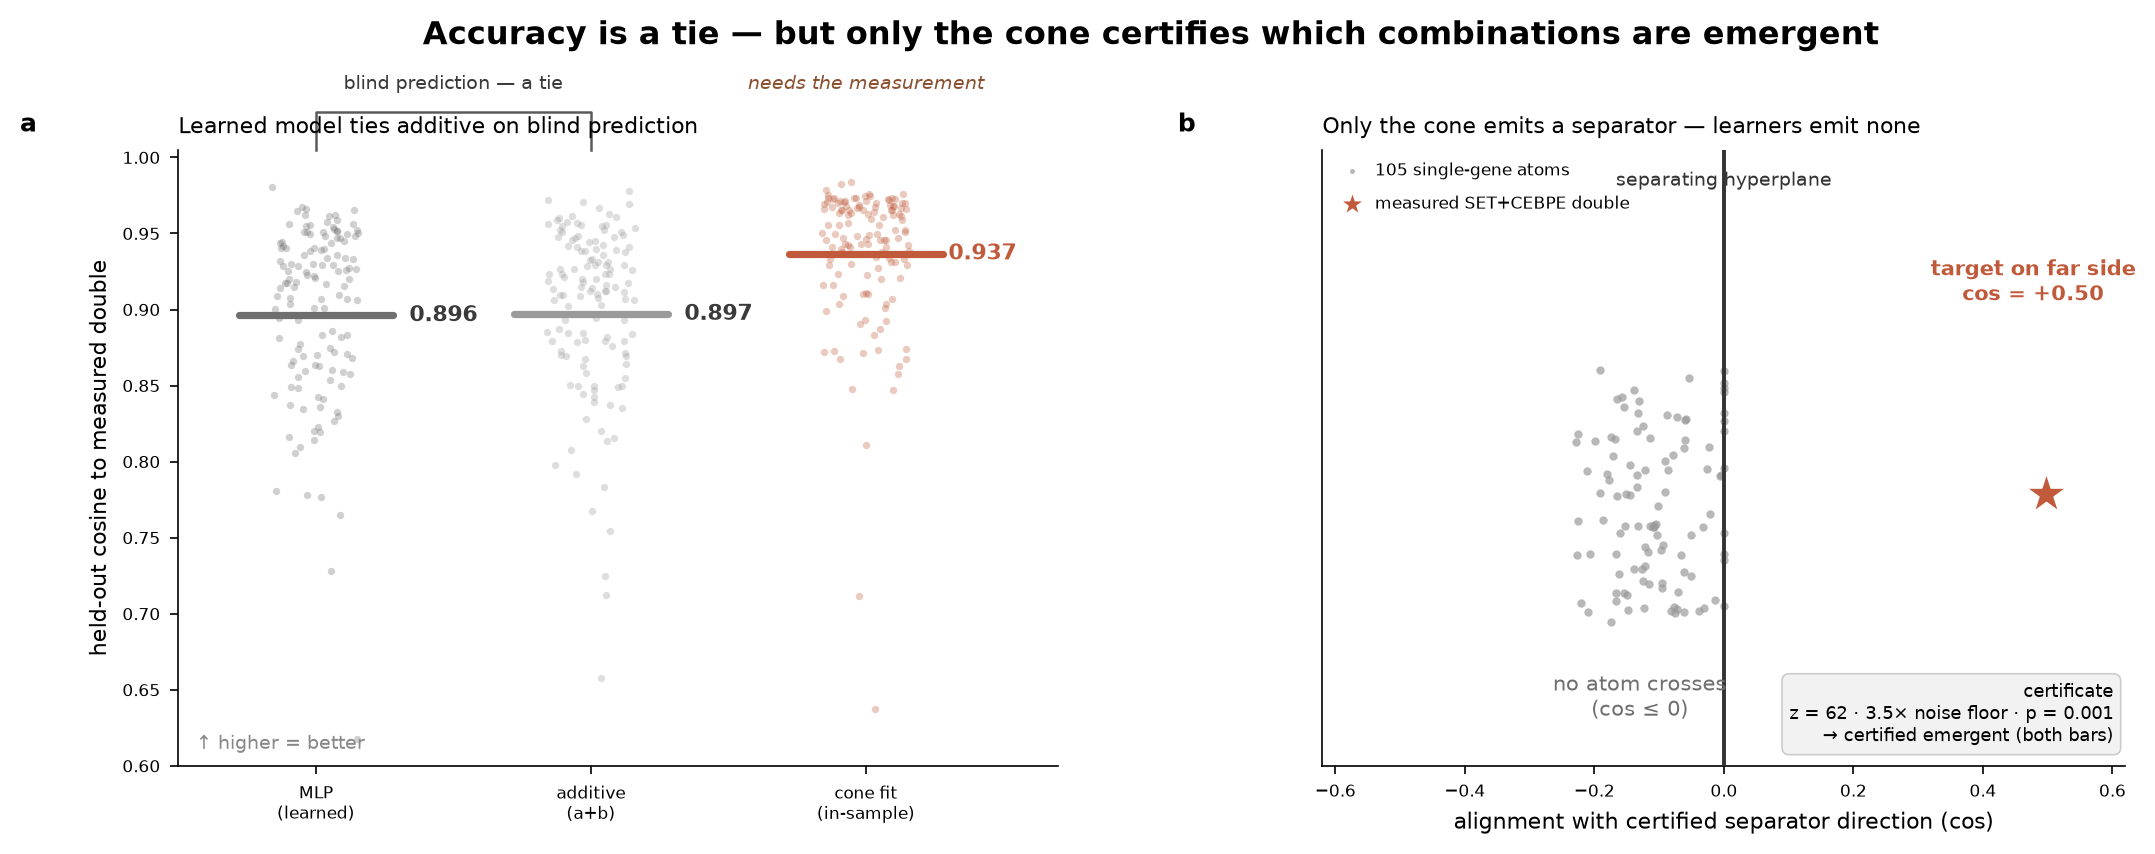
\includegraphics[width=\textwidth]{fig1_hook.png}
\caption{\textbf{Accuracy is a tie---but only the cone certifies which combinations are emergent.}
\textbf{(a)} Blind (leave-pairs-out) prediction of $131$ measured Norman doubles: a self-contained
learned MLP (mean held-out cosine $0.896$) is indistinguishable from the trivial additive baseline
($0.897$); the cone's higher in-sample number ($0.937$) requires seeing the measurement and is not
a forecast. \textbf{(b)} For one certified pair (SET$+$CEBPE), the Farkas/KKT separator places all
$105$ single-gene atoms on one side ($\cos\le 0$) and the measured double strictly on the other
($\cos=+0.50$); the learned and additive predictors emit no such certificate on any of the $131$
outside-cone doubles. $n=131$ doubles; unit of replication is the perturbation pair.}
\label{fig:hook}
\end{figure*}

Figure~\ref{fig:hook} states the paper's thesis as data. A learned model and a one-line additive
rule predict held-out combination effects equally well, so predictive accuracy cannot be the
criterion for calling a combination special. What distinguishes the convex-cone view is not
accuracy but a falsifiable output: for every combination whose measured effect leaves the
single-gene cone, the same convex program returns a separating hyperplane certifying the
unreachable direction. The rest of this section builds that certificate, makes it robust to
measurement noise, turns it into a training-free triage rule, and shows it generalizes across
interaction order and across screens.

\begin{figure*}[t]
\centering
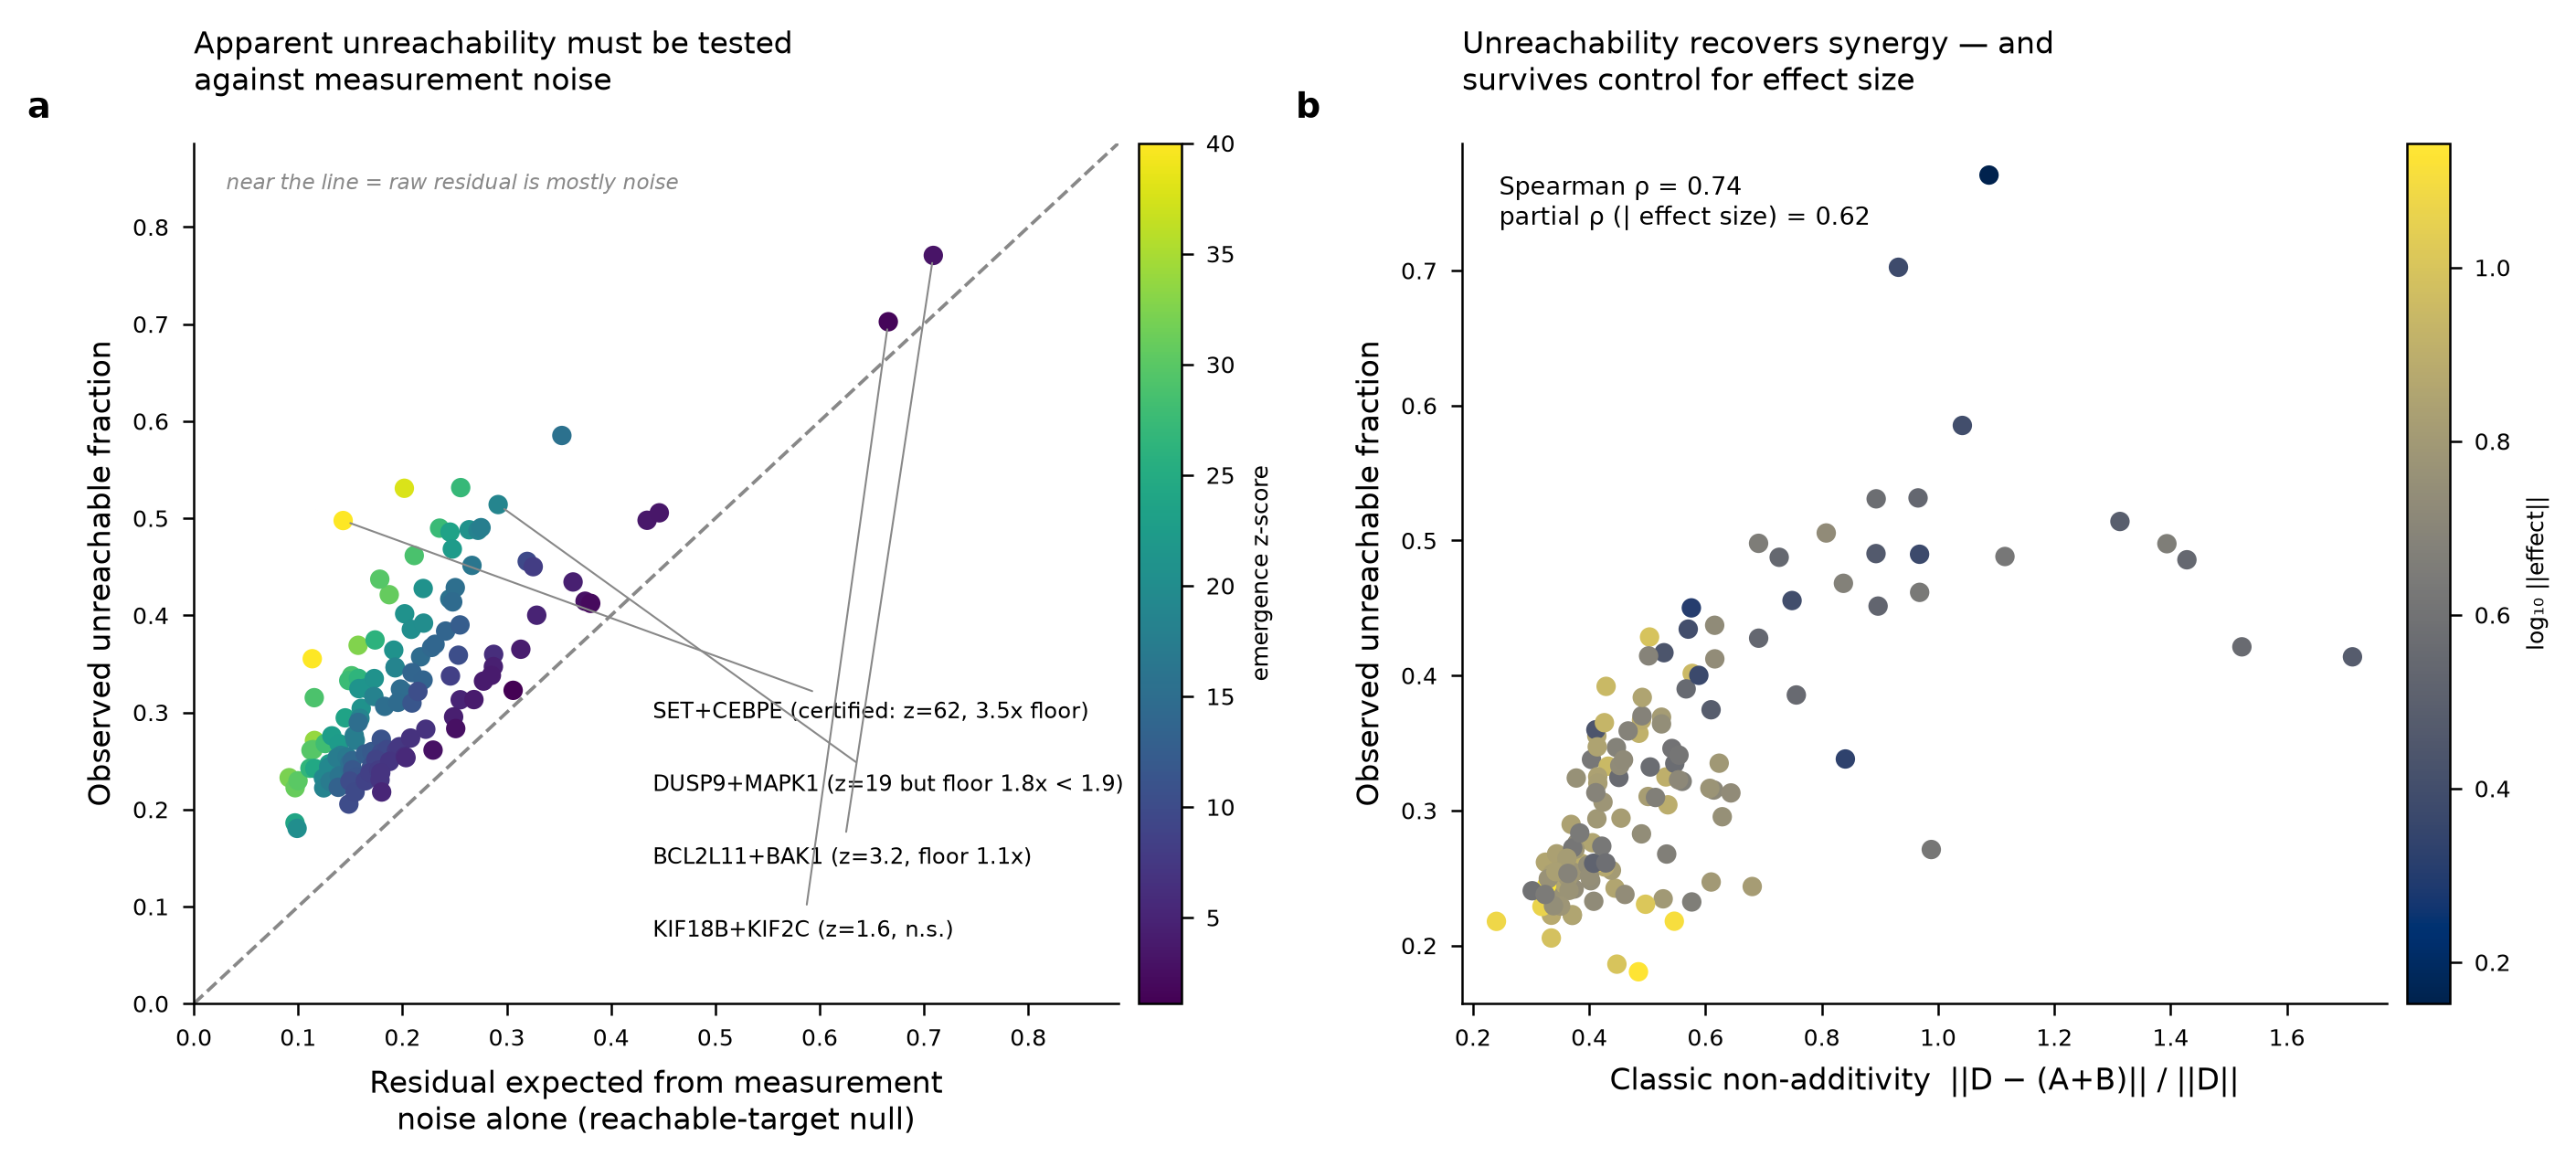
\includegraphics[width=\textwidth]{fig2.png}
\caption{\textbf{The emergence certificate must clear a measurement-noise bar.}
\textbf{(a)} For each of $131$ Norman doubles, observed unreachable fraction (y) against the
residual expected from measurement noise alone under the reachable-target null (x); points near
the diagonal are consistent with noise. Colour is the noise-aware emergence $z$. \textbf{(b)} The
noise-aware certificate recovers classical synergy: observed residual against the non-additivity
score $\lVert\dvec-(\mathbf{a}+\mathbf{b})\rVert/\lVert\dvec\rVert$ (Spearman $0.74$; partial
Spearman $0.62$ controlling for effect magnitude, shown by colour). $129/131$ clear bar~(a)
($p<0.05$); $35/131$ also clear bar~(b) ($1.9\times$ floor). $n=131$ doubles.}
\label{fig:certificate}
\end{figure*}

\subsection{The certificate, and the noise bar it must clear}
\label{sec:results-certificate}

On the Norman combinatorial CRISPRa screen (data file labelled A549; canonical line K562), we
build a dictionary of $105$ single-gene effect vectors over $5{,}045$ genes and project each of
$131$ measured doubles onto their non-negative cone (Section~\ref{sec:methods-cone}). Every one of
the $131$ doubles lies geometrically outside the cone: no non-negative mixture of the measured
singles reproduces the measured double, and each carries a Farkas/KKT separator at machine
precision.

Geometric ``outside,'' however, is not yet evidence of emergence. Because the unreachable fraction
is normalized by target norm, a small-magnitude double measured with the same absolute noise as a
large one shows an inflated apparent residual. The raw unreachable fraction indeed tracks effect
magnitude at Spearman $-0.56$ ($p=4\times10^{-12}$), and only a minority of doubles clear their own
split-half noise floor (Fig.~\ref{fig:certificate}a). We therefore replace the point residual with
a noise-injection null (Section~\ref{sec:methods-null}): starting from the reachable fit
$\hat{\dvec}$, we add per-gene Gaussian noise calibrated to the split-half standard error and ask
how far outside the cone a genuinely reachable target would appear under that noise, repeating
$B=200$ times. The resulting $z$-score and plus-one empirical $p$ quantify emergence above
measurement noise, and---critically---no longer track magnitude (Spearman $+0.14$, $p=0.13$;
Fig.~\ref{fig:certificate}b).

This yields a two-bar verdict. Bar~(a), the permissive significance test, is cleared by $129/131$
doubles at $p<0.05$. Bar~(b), a stricter requirement that the residual exceed $1.9\times$ its own
noise floor, is cleared by $35/131$. We report both because they answer different questions: bar~(a)
asks whether a double is emergent at all above noise; bar~(b) asks whether the emergence is large
relative to how noisily it was measured. The most strongly certified pairs are
SET$+$CEBPE ($z=62$, floor ratio $3.5\times$), IRF1$+$SET ($z=49$), and MAPK1$+$PRTG ($z=38$), each
clearing both bars; the classical DUSP9$+$MAPK1 phosphatase-substrate synergy is strongly
significant ($z=19$) but sits just below the bar~(b) floor ($1.8\times<1.9\times$), a reminder that
the two bars are distinct. A textbook
apoptosis pair, BCL2L11$+$BAK1, passes bar~(a) only weakly ($z=3.2$, $p=0.002$) and does not clear
bar~(b), and the mitotic pair KIF18B$+$KIF2C is the one headline pair that fails significance
($z=1.6$, $p=0.055$)---the noise bar demoting exactly the pairs whose apparent unreachability was a
magnitude artefact. Reassuringly, the noise-aware certificate recovers classical non-additivity:
the observed residual correlates with the standard synergy score $\lVert\dvec-(\mathbf{a}+\mathbf{b})\rVert/\lVert\dvec\rVert$
at Spearman $0.74$, and at partial Spearman $0.62$ after controlling for effect magnitude
(Fig.~\ref{fig:certificate}b), so the signal is synergy, not scale.

\begin{figure*}[t]
\centering
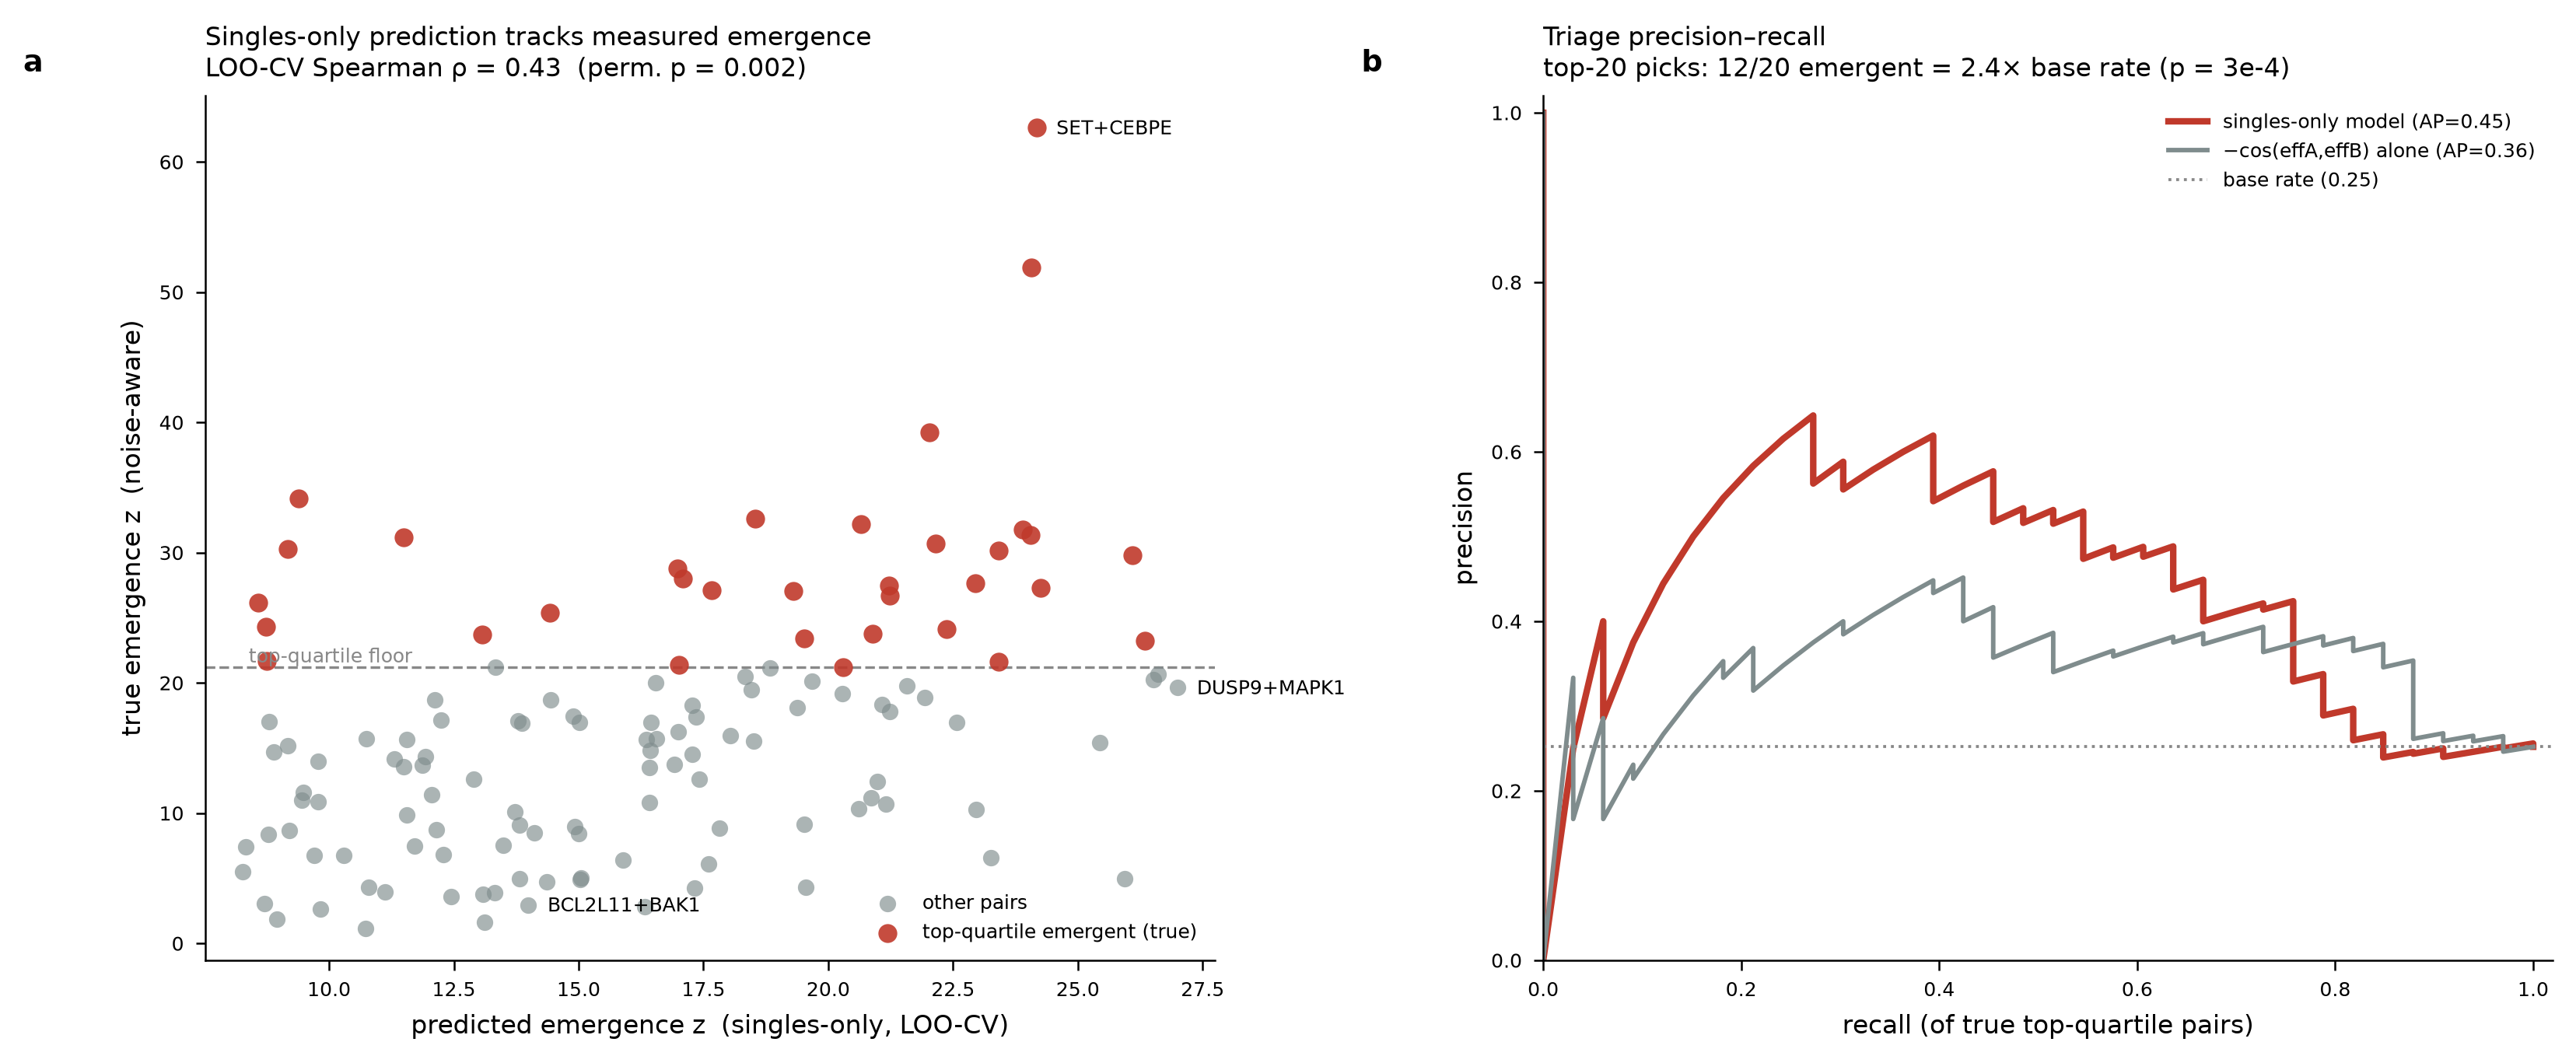
\includegraphics[width=\textwidth]{fig3.png}
\caption{\textbf{Training-free triage of unmeasured combinations.}
\textbf{(a)} Singles-only predicted emergence (leave-one-out) against measured noise-aware $z$;
Spearman $0.43$ (permutation $p=0.002$). \textbf{(b)} Precision--recall for flagging true
top-quartile emergent pairs: the top $20$ picks by the training-free score contain $12$ emergent
($2.4\times$ the $0.25$ base rate, $p=3\times10^{-4}$). The single-scalar $-\cos(\mathbf{a},\mathbf{b})$
alone (grey) already beats the base rate; a ridge model on a small labelled pilot (red) adds little
and is reported only as a ceiling. $n=131$ doubles.}
\label{fig:triage}
\end{figure*}

\subsection{Training-free triage of unmeasured combinations}
\label{sec:results-triage}

The certificate needs the measured combination. The complementary question---which of the
$\binom{n}{2}$ unmeasured combinations to run---must be answered from singles alone. We find that a
single scalar predicts emergence prospectively: the negative cosine between the two single-gene
effect vectors, $-\cos(\mathbf{a},\mathbf{b})$. Pairs of dissimilar singles are more likely to
produce an emergent combination (Spearman between $-\cos$ and the raw unreachable label $-0.47$;
against the noise-aware label $-0.37$). Ranking the $131$ doubles by this training-free score and
taking the top $20$ recovers $12$ true top-quartile emergent pairs---a $2.4\times$ enrichment over
the $0.25$ base rate ($p=3\times10^{-4}$; Fig.~\ref{fig:triage})---or $7/20$, a $1.4\times$
enrichment, against the stricter noise-aware label. A supervised ridge model on a small labelled
pilot (nine singles-only features, leave-one-out) reaches Spearman $0.43$ (permutation $p=0.002$),
a modest ceiling that we report in supplement; the headline triage claim needs no training data at
all.

\begin{figure*}[t]
\centering
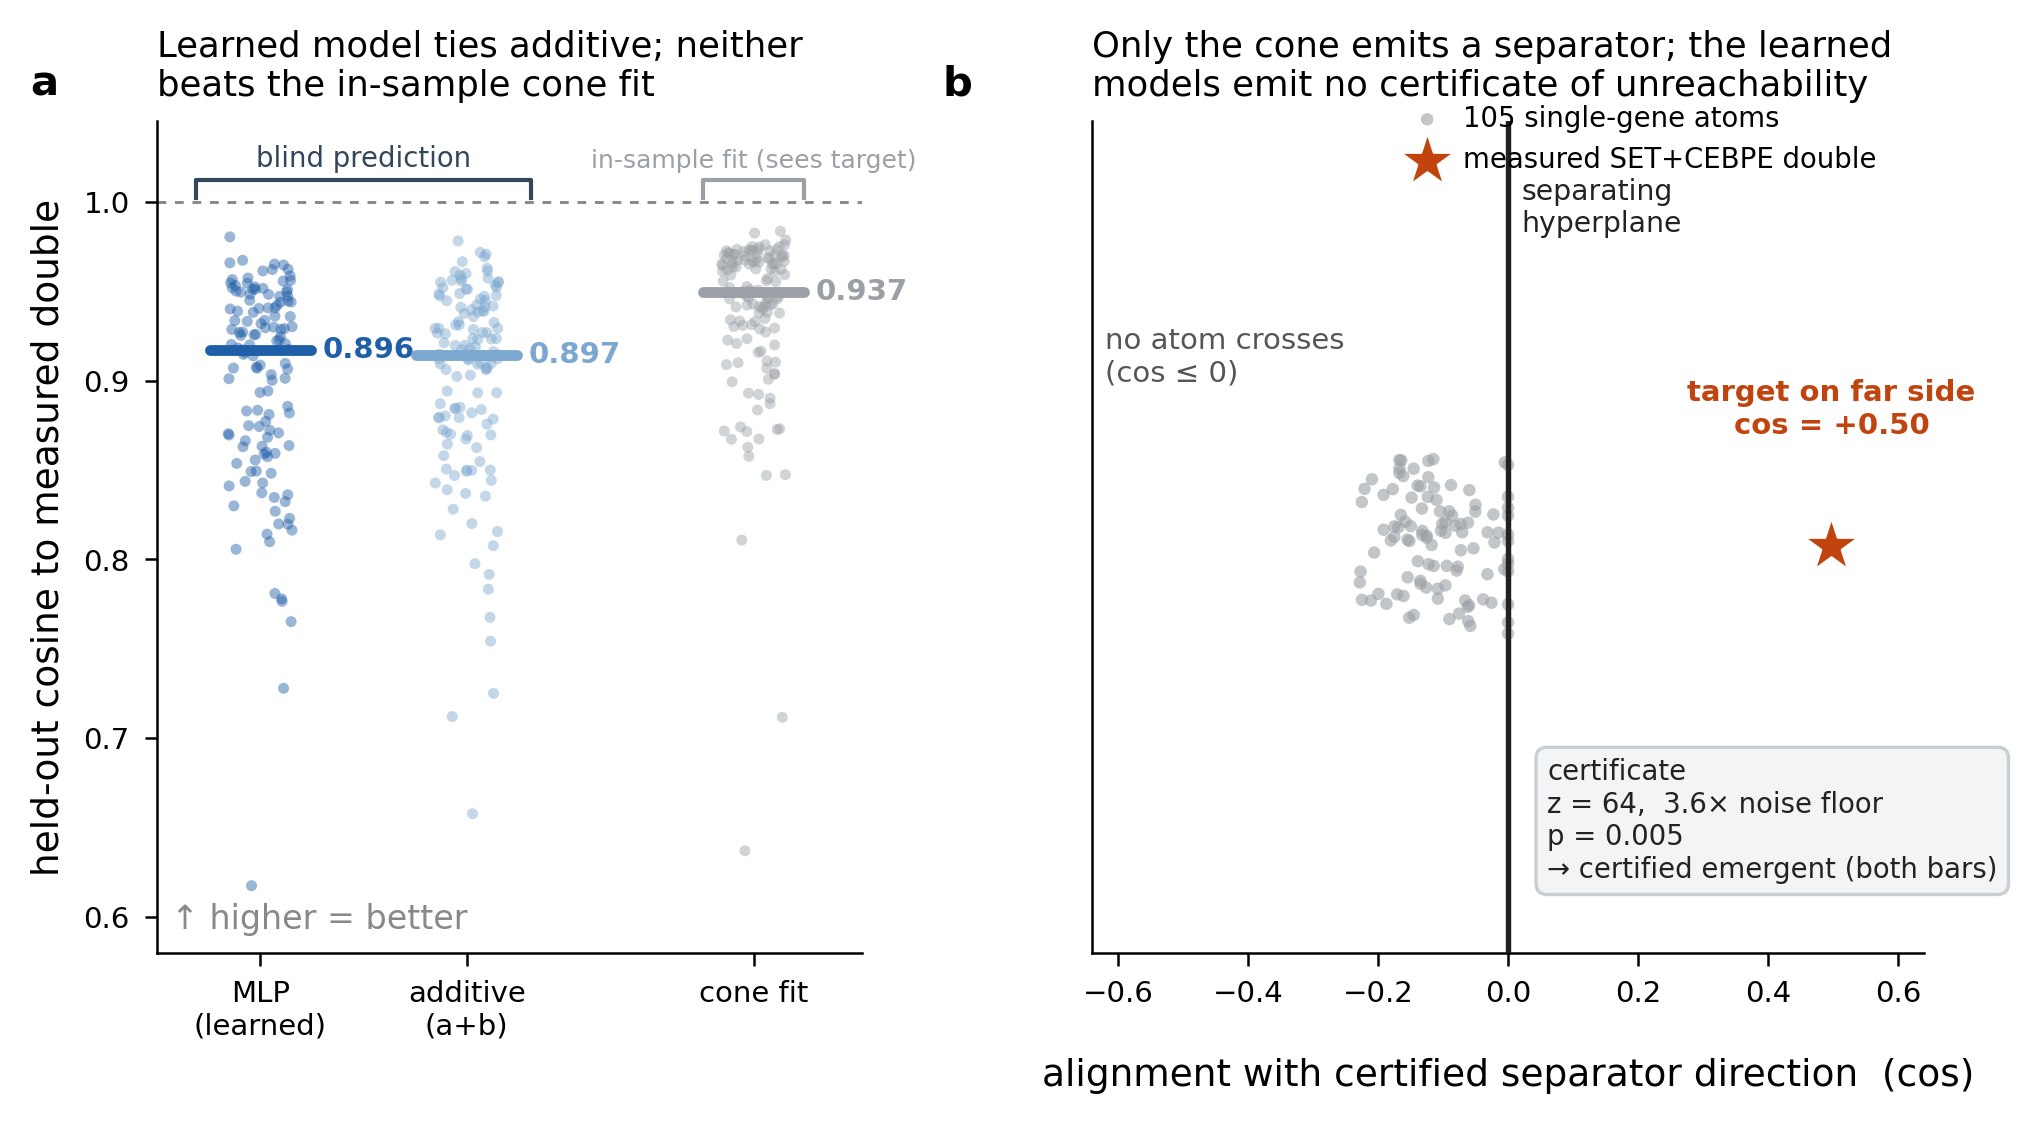
\includegraphics[width=\textwidth]{fig4.png}
\caption{\textbf{Head-to-head: a learned model ties additive, and neither certifies.}
\textbf{(a)} Leave-pairs-out blind prediction of $131$ measured doubles: the learned MLP (mean
cosine $0.896$) ties the additive baseline ($0.897$); the cone's in-sample fit ($0.937$) requires
the measured double and is not a blind forecast. \textbf{(b)} For a certified pair, only the cone
emits a separating hyperplane: all $105$ single atoms fall on one side ($\cos\le0$) and the
measured double on the other; the learned and additive predictors emit no certificate on any of
the $131$ outside-cone doubles. $n=131$ doubles.}
\label{fig:headtohead}
\end{figure*}

\subsection{Head-to-head against a learned baseline}
\label{sec:results-headtohead}

To test whether a learned interaction model changes the picture, we built a self-contained neural
baseline with no external dependencies: an additive-anchored two-layer MLP (hidden width $32$,
trained on a $50$-component SVD of the $105$ atoms retaining $95.6\%$ of atom-span variance) that
predicts a double's effect from its two single effects, evaluated leave-pairs-out on all $131$
doubles. Its blind held-out cosine is $0.896$, statistically tied with the additive baseline's
$0.897$ (the MLP wins on $49.6\%$ of doubles), reproducing the 2025--2026 result that learned
perturbation models do not beat additivity out-of-sample \citep{AhlmannEltze2025}. The cone's
in-sample reconstruction cosine ($0.937$) is higher but is not a blind forecast---it requires the
measured double. The head-to-head (Fig.~\ref{fig:hook}, expanded in Fig.~\ref{fig:headtohead})
makes the paper's central point precise: on the metric the field optimizes, the methods tie; on the
output that supports a decision---a per-pair certificate of unreachability---only the cone delivers,
emitting a valid separator on all $131$ outside-cone doubles where both predictors emit none.

\begin{figure*}[t]
\centering
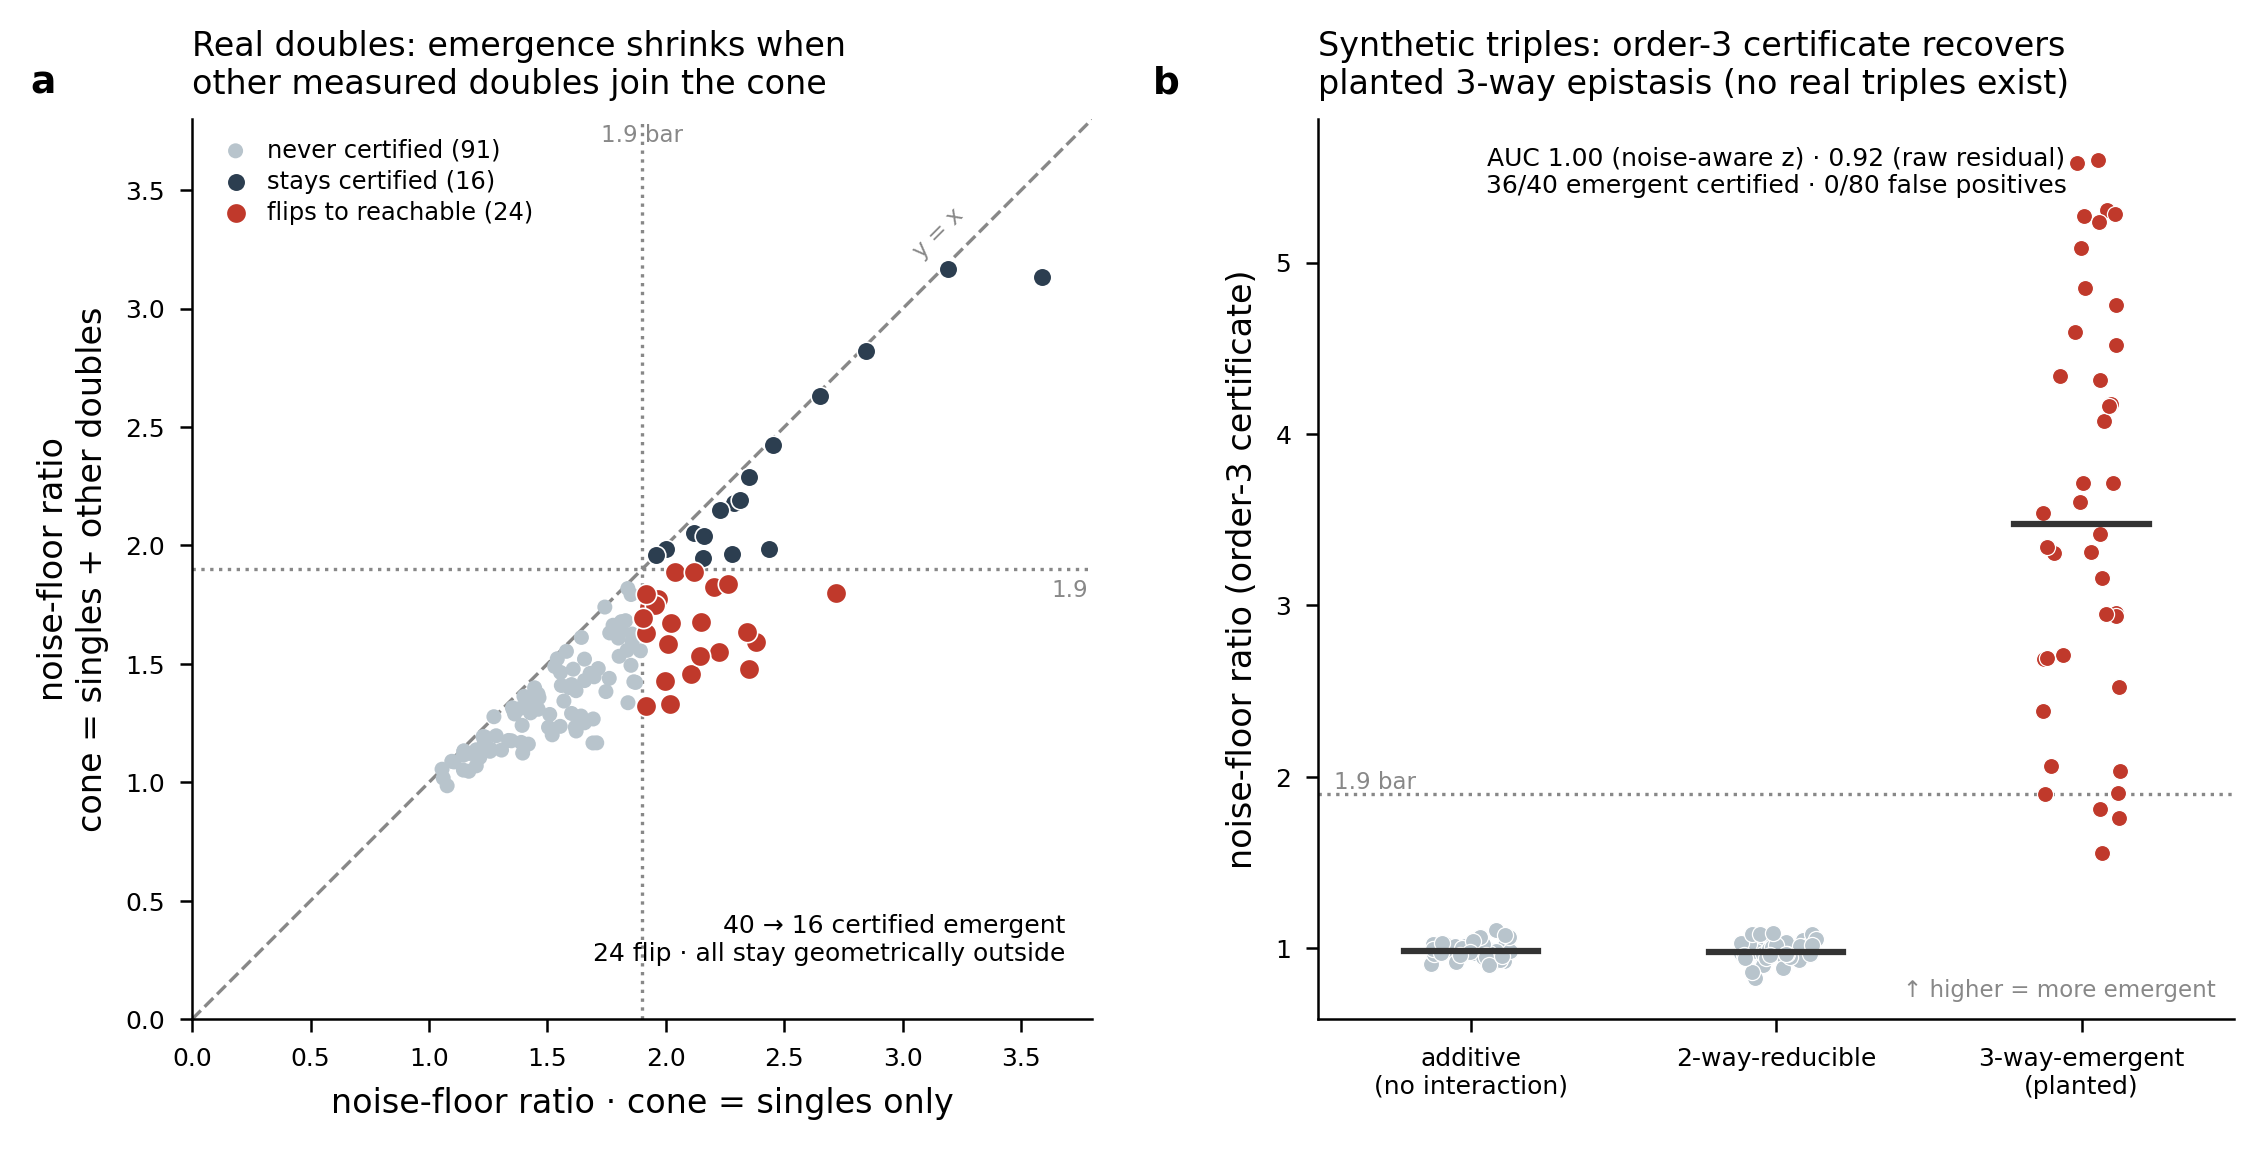
\includegraphics[width=\textwidth]{fig5.png}
\caption{\textbf{The certificate generalizes to interaction order $k$.}
\textbf{(a)} Real Norman doubles: noise-floor ratio against the single-gene cone (x) versus against
the enlarged cone of singles-plus-other-doubles (y). Enlarging the reference set shrinks the
certified-emergent set from $40$ to $16$; $24$ doubles flip from emergent to reachable, while all
$131$ remain geometrically outside both cones. \textbf{(b)} Synthetic planted-epistasis triple
screen (the Norman screen measures no triples): the order-$3$ certificate separates planted
$3$-way-emergent triples from additive and $2$-way-reducible ones at AUC $1.00$ (noise-aware $z$),
certifying $36/40$ emergent triples with $0/80$ false positives.}
\label{fig:kway}
\end{figure*}

\subsection{The certificate generalizes to interaction order $k$}
\label{sec:results-kway}

Emergence is not restricted to pairs. The cone construction generalizes verbatim to order $k$: to
ask whether an order-$k$ combination is emergent \emph{relative to everything of lower order}, we
project its measured effect onto the cone spanned by all lower-order effects. On real data this
sharpens the verdict. When the single-gene cone is enlarged with the other measured doubles (from
$105$ to $235$ atoms), the number of certified-emergent doubles shrinks from $40$ to $16$: $24$
pairs that look emergent against singles alone become reachable once other measured doubles enter
the dictionary (Fig.~\ref{fig:kway}a). All $131$ doubles nonetheless remain geometrically outside
both cones; the shrinkage is driven by effect size crossing the noise bar, not by a change in
geometric membership---emergence is a property of the reference set, and the method makes that
reference explicit. Because the Norman screen measures no triples, we validate the order-3 code path
on a synthetic planted-epistasis screen with known ground truth: the order-3 certificate recovers
planted $3$-way-emergent triples from additive and $2$-way-reducible ones at AUC $1.00$ on the
noise-aware score ($0.92$ on the raw residual), certifying $36/40$ true emergent triples with $0/80$
false positives (Fig.~\ref{fig:kway}b). This is a validation of the machinery, not a claim about
biological $3$-way epistasis, which the data cannot support.

\begin{figure*}[t]
\centering
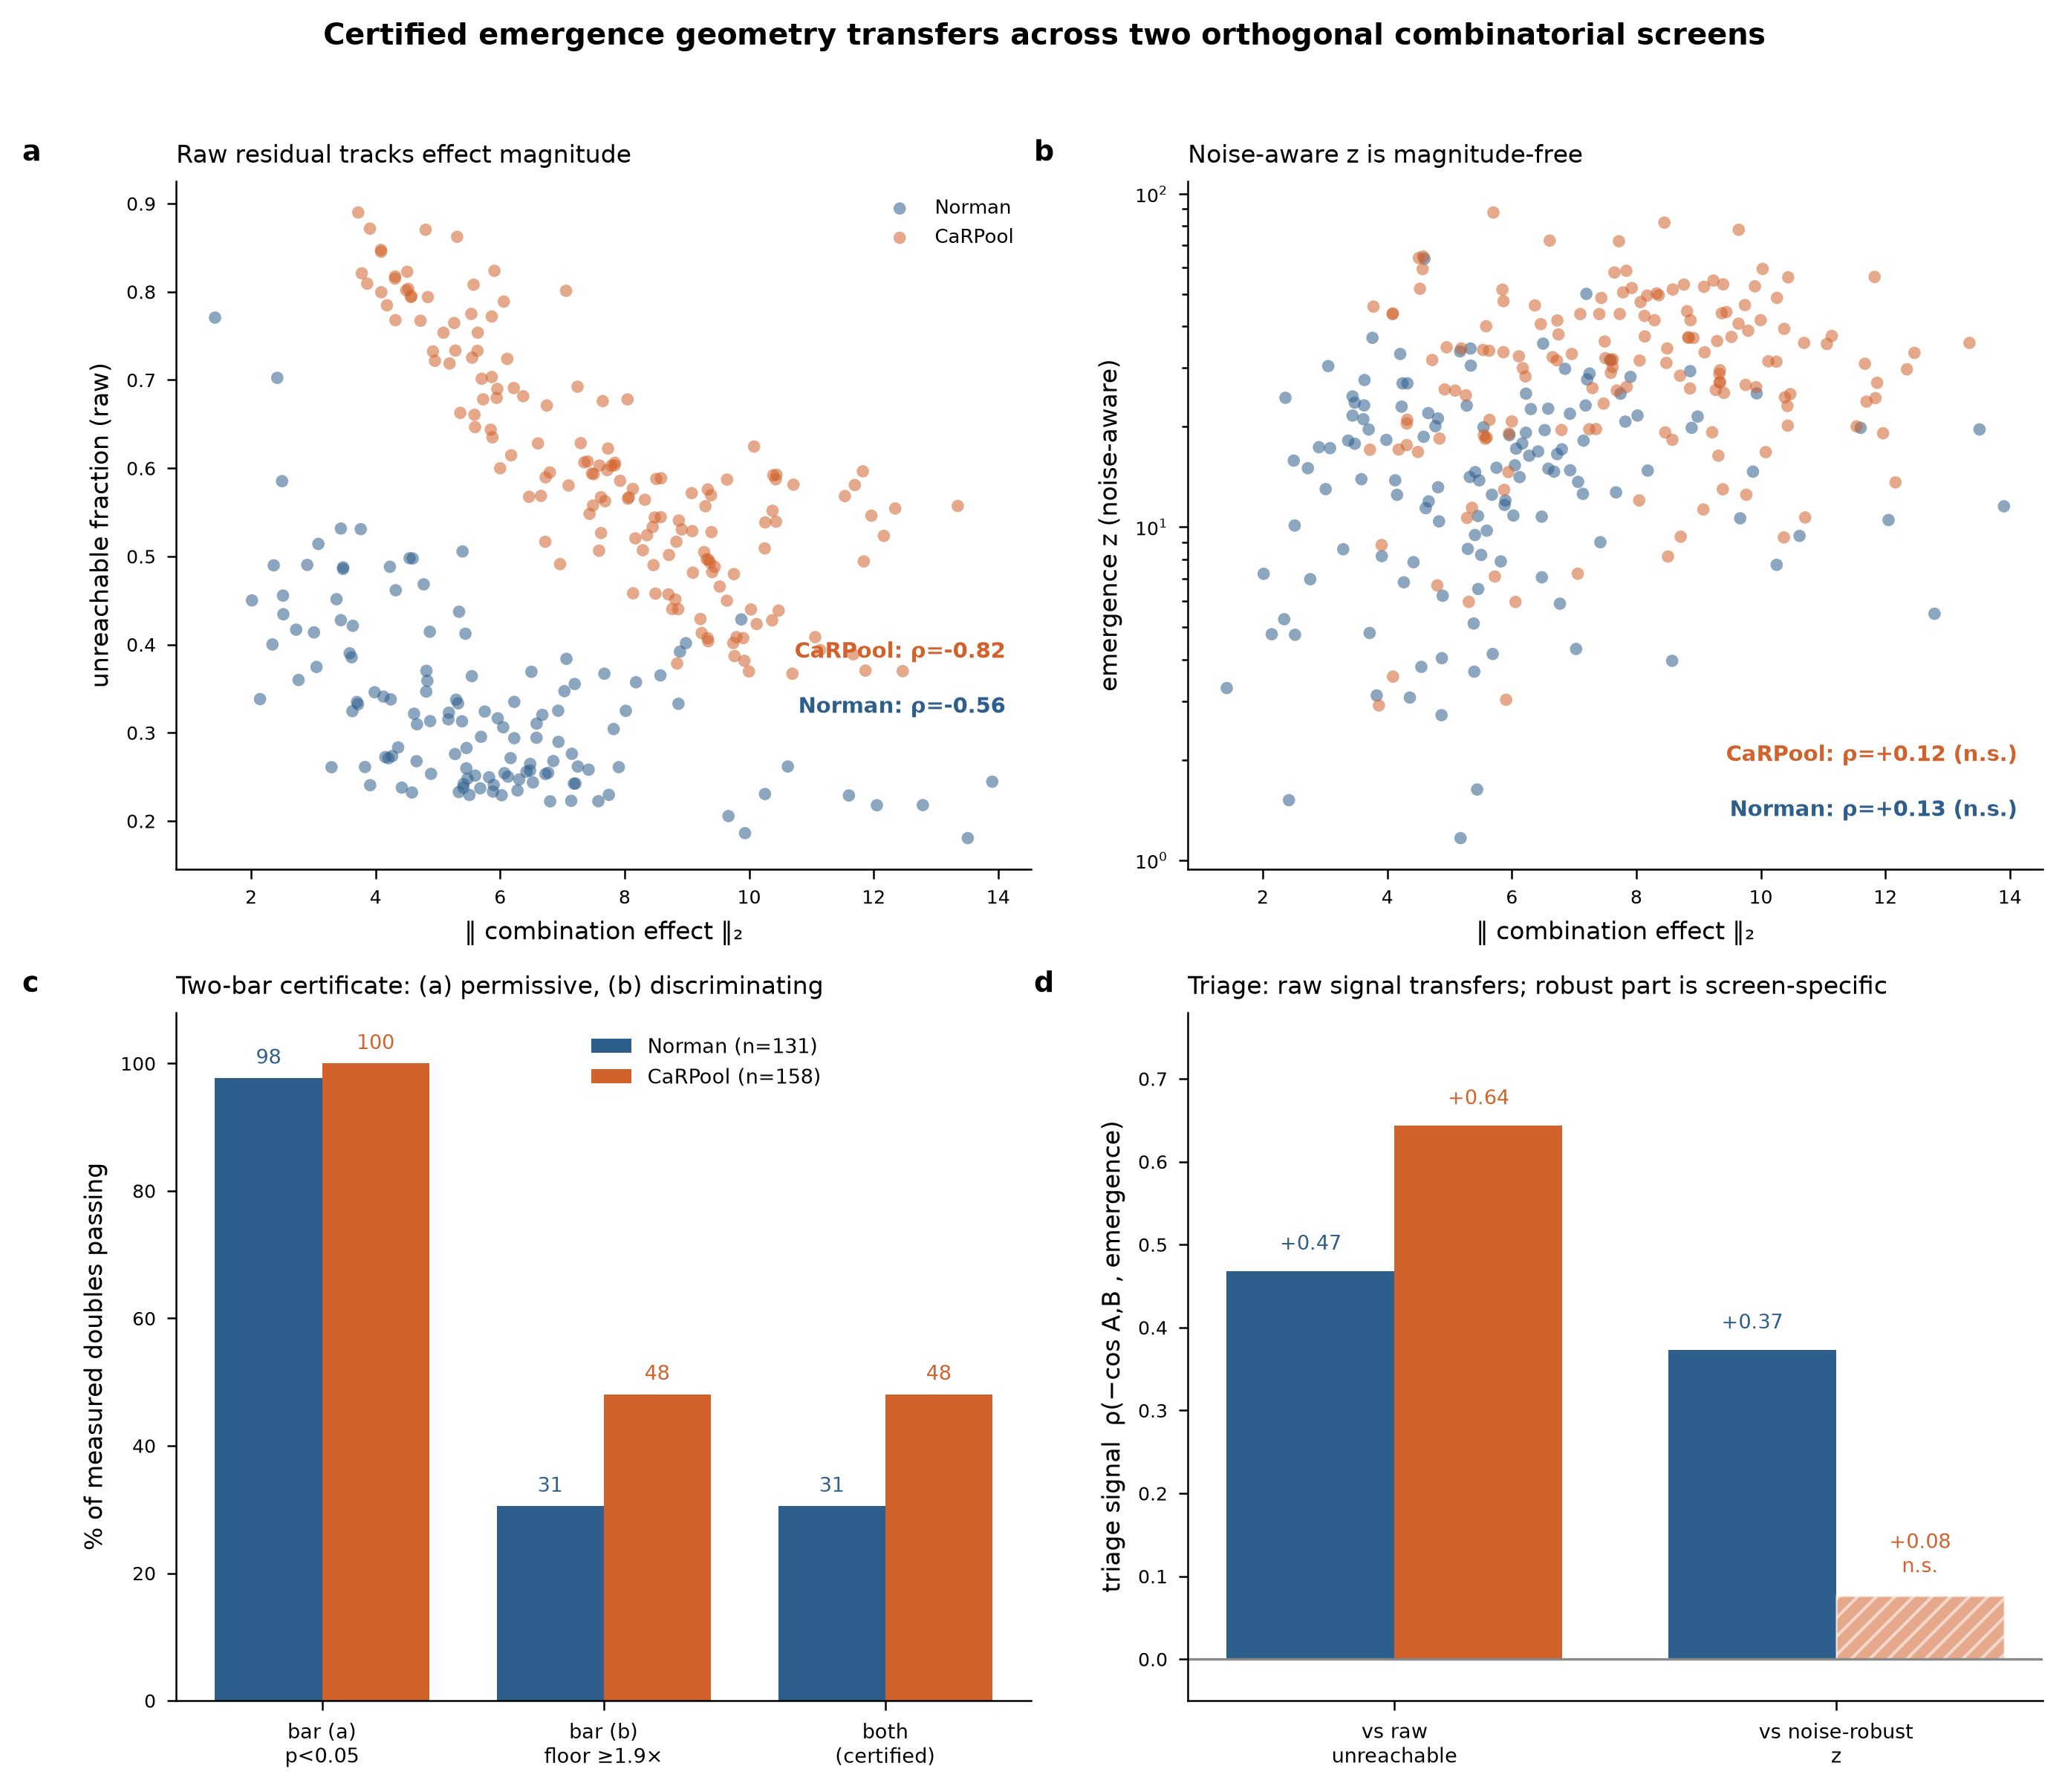
\includegraphics[width=\textwidth]{fig6.png}
\caption{\textbf{The certificate and its noise discipline transfer to an orthogonal screen.}
Norman CRISPRa doubles (blue) and CaRPool-seq Cas13d-knockdown doubles in THP-1 (orange).
\textbf{(a)} Raw unreachable fraction tracks effect magnitude in both screens ($-0.56$, $-0.82$).
\textbf{(b)} The noise-aware $z$ is magnitude-free in both ($+0.14$, $+0.12$). \textbf{(c)} The
two-bar certificate reproduces (CaRPool $48\%$ certified, Norman $31\%$ under the shared symmetric
pipeline). \textbf{(d)} The training-free triage rank transfers against the raw label
($\sim\!2.2\times$ in both) but its magnitude-controlled component is screen-specific (survives in
Norman, not significant in CaRPool). $n=131$ (Norman), $158$ (CaRPool) doubles.}
\label{fig:crossscreen}
\end{figure*}

\subsection{The certificate transfers to an orthogonal screen}
\label{sec:results-crossscreen}

Finally, we ask whether the emergence geometry is a property of one screen or of combinatorial
perturbation data generally. We repeat the entire pipeline on CaRPool-seq \citep{Wessels2023}, a
Cas13d RNA-targeting knockdown screen in THP-1 cells---orthogonal to Norman in perturbation modality
(knockdown vs.\ CRISPRa activation), direction, target molecule, and cell line---with $28$ single
atoms and $158$ measured doubles. Three findings transfer (Fig.~\ref{fig:crossscreen}). First, the
magnitude confound is universal: the raw unreachable fraction tracks effect magnitude in both
screens ($-0.56$ Norman, $-0.82$ CaRPool), and the noise-aware $z$ removes it in both ($+0.14$,
$+0.12$). Second, the two-bar certificate reproduces, with CaRPool showing a higher certified
fraction ($76/158$, $48\%$) than Norman ($40/131$ under the shared pipeline). Third, the
training-free triage rank transfers against the raw label ($\sim\!2.2\times$ enrichment in both),
but its magnitude-controlled component is screen-specific: the noise-robust triage correlation
survives in Norman (Spearman $0.37$) and is not significant in CaRPool ($0.08$). The certificate and
its noise discipline generalize; the prospective triage rule generalizes in rank but should be
recalibrated per screen---an honest boundary we state rather than paper over.


% Related work section fragment — natbib \citep/\citet; no preamble.
% Every citation key resolves to an entry in references.bib.
\section{Related work}
\label{sec:related}

Cell-state engineering poses an inverse-design question: given a starting state and a
desired target state, which interventions move the cell there, and is the move even
possible? This is the question behind directed differentiation, transdifferentiation, and
T-cell engineering, and it is the question of pharmaceutical target selection. Getting it
wrong is the dominant cost of drug development: only about one in ten clinical programmes
reaches approval, and failure is paid for late \citep{Minikel2024,WongSiahLo2019}. Attrition concentrates
at Phase~II, and roughly half of Phase~II/III failures are for lack of efficacy---the
wrong target or mechanism rather than safety \citep{Harrison2016}. The two interventions
with published evidence of improving those odds both point the same way: human genetic
support raises the odds of approval about 2.6-fold \citep{Minikel2024,Nelson2015}, and
\emph{measured} rather than inferred target effects are the direct antidote to the
11--25\% preclinical reproducibility documented by the Amgen and Bayer audits
\citep{BegleyEllis2012,Prinz2011}. A method for this problem should therefore (i)~work from
measured effects in the relevant cell type, (ii)~answer achievability rather than merely
rank candidates, and (iii)~say so honestly when a goal is not achievable.

We surveyed 91 prior methods spanning 2011--2026 (92 including this work) across
control-theoretic network control,
gene-regulatory-network (GRN) inference with in-silico perturbation, deep
perturbation-response prediction, single-cell foundation models, and the
combinatorial-screen, optimal-transport, virtual-cell, and benchmark literature that
borders them. Positioning them on two axes---\emph{what question is answered} (forward
prediction versus feasibility) and \emph{what the answer is grounded in} (an inferred or
hand-built model versus directly measured effects)---exposes a gap that is exact rather
than rhetorical. The methods grounded in measured effects answer only forward questions,
and the methods that reason about feasibility do so only inside a model.

\paragraph{Model-theoretic feasibility.}
The most mature theory for the intervention question is network control. Structural and
target controllability cast steering an assumed linear system as a matching problem over
network topology \citep{Liu2011,Gao2014}, and determining-node / control-kernel methods
identify driver sets from structure \citep{Mochizuki2013,Kim2013}. Boolean attractor
control computes node interventions that switch a logical network between attractors
\citep{Zanudo2015,Zanudo2017,Joo2018,Marazzi2022}, a line that remains active
\citep{Cifuentes-Fontanals2025,Metzcar2025,Murrugarra2025,Trinh2025,Vecchio2026}. A
data-fitted strand fits a dynamical model to omics and then applies control theory
\citep{Ronquist2017,Rukhlenko2022,Wytock2024}, and network-influence predictors rank
transcription-factor sets for a conversion \citep{Rackham2016,Cahan2014}. These are the
methods that carry a controllability or control-strategy guarantee---but the guarantee is
a property of a hand-built, fitted, or inferred model, never of measured effects, and the
control set is only as trustworthy as the network put in. The same dependency reappears
whenever feasibility-style reasoning is imported onto a reconstructed single-cell GRN
\citep{Wang2023CEFCON} or run in a learned latent space \citep{Han2025}. The set of prior
methods that emit any verdict- or certificate-like output is therefore not one family: it
spans structural and Boolean network control, control-from-data, an inferred single-cell
GRN, and one causally inspired perturbation predictor. What unites them is the assumed
model, not the family.

\paragraph{Measured-grounded forward prediction.}
The single-cell community answers the same biological question by running an inferred
network forward. CellOracle infers a GRN and simulates a transcription-factor knockout
into predicted identity transitions \citep{Kamimoto2023}; related tools infer regulons,
enhancer networks, or dynamic GRNs \citep{Aibar2017,Xu2021,BravoGonzalezBlas2023,%
Wang2023Dictys,Osorio2022}, with BEELINE quantifying how method-dependent GRN inference
is \citep{Pratapa2020}. Deep perturbation-response models are genuinely
measured-grounded---they learn from real Perturb-seq data---but are resolutely forward:
GEARS predicts outcomes of unseen multi-gene perturbations \citep{Roohani2023}, and
compositional and disentanglement models predict responses to given perturbations
\citep{Lotfollahi2019,Lotfollahi2023,Hetzel2022,Piran2024}. Single-cell foundation models
\citep{Theodoris2023,Cui2024,Hao2024} and the 2025--2026 virtual-cell surge---perturbation
transformers, atlas-scale models and challenges, and giga-scale perturbation atlases
\citep{Adduri2025,Roohani2025,Zhang2025Tahoe,Klein2025b}---extend the same forward map.
Optimal-transport methods describe how cells \emph{do} move rather than which interventions
\emph{would} move them \citep{Schiebinger2019,Lange2022}, and experimental-design methods
choose the next screen \citep{Huang2024}. Every one maps perturbation to predicted
response: a predictor always returns \emph{some} answer and structurally cannot certify
that a target is unreachable.

\paragraph{Why a feasibility verdict, not another predictor.}
A cluster of 2025--2026 benchmarks reports that current perturbation-prediction models,
foundation models included, often fail to beat simple mean or linear baselines on
genuinely unseen perturbations \citep{AhlmannEltze2025,Wong2025,Csendes2025,%
Kedzierska2025,Wu2025,Vinas2025,Kernfeld2025,Wei2025,Luecken2025,Atti2025,Mao2026,%
Vollenweider2026}. This is the field's own critique, and it sharpens the case for a
different output: a feasibility verdict computed directly from measured effects does not
extrapolate to unseen perturbations at all, and it comes with a checkable certificate and a
shuffled-target null. The claim is deliberately weaker, and therefore more defensible, than
predicting an unseen response.

\paragraph{Our position.}
Across all 91 prior methods (ours excluded), 14 operate directly on measured effects---and
all 14 only predict or rank; \emph{none} returns a feasibility verdict, emits a
data-grounded certificate, or proves infeasibility, and the 13--15 partial verdict/%
certificate marks are all model-theoretic. The two capabilities this work
combines---measured grounding and a feasibility verdict with a certificate---are held by
\emph{disjoint} sets of prior methods, and their intersection is empty. We compose the
measured genome-scale CRISPRi effect vectors from a Perturb-seq screen in primary human
CD4$^+$ T cells \citep{Zhu2025} directly, with no inferred network. Because knockdown is
loss-of-function and combinations are non-negative, reachability becomes membership in a
convex cone, solved by non-negative least squares \citep{LawsonHanson1974}: ``reachable''
returns the mixing weights (a minimal ranked recipe), and ``outside the cone'' is a theorem
whose separating hyperplane---a Farkas/KKT certificate \citep{Farkas1902}---names the genes
that would have to be \emph{activated} instead, a falsifiable CRISPRa hypothesis rather than
a null result. We validate by held-out-gene generalisation against a shuffled-target null
(Th2$\rightarrow$Th1 held-out cosine $0.448$, null $z\approx24$; KKT residual
$\approx\!10^{-11}$), and the operator transfers unchanged to the Norman K562 combinatorial
CRISPR screen \citep{Norman2019} (held-out CEBPA cosine $0.878$), whose measured
double-perturbations show that the additivity assumption is a bounded approximation (median
cosine $0.71$, sum-of-singles versus measured) rather than exact. We claim novelty for this
measured-effect, certificate-carrying reachability \emph{decision}, not for the T-cell or
CEBPA regulator lists, which the source screens \citep{Zhu2025,Norman2019} already report
and which we use only as positive controls; activation hypotheses require a separate CRISPRa
arm \citep{Schmidt2022}, and the modest absolute cosine is the ceiling of
loss-of-function alone.


\section{Discussion}
\label{sec:discussion}

We have described a certified triage instrument for combinatorial perturbation screens. It treats
a screen's single-gene effect vectors as a dictionary and decides, by convex geometry, whether a
measured combination reaches a cell-state direction that the singles cannot---answering ``is this
combination emergent?'' with a Farkas/KKT certificate rather than a prediction, and answering
``which unmeasured combinations are worth running?'' with a training-free score computed from the
singles alone. The value of the framework is not a new list of synergistic gene pairs---those are
already in the source screens and we use them only as positive controls---but a new \emph{kind of
output}: a falsifiable, noise-aware emergence certificate computed directly from measured effects,
which no forward predictor supplies.

\subsection{Interpretation}
The central methodological finding is that predictive accuracy is the wrong axis for claiming a
combination is special. A self-contained learned model and a one-line additive rule predict
held-out double effects equally well ($0.896$ vs.\ $0.897$), consistent with a wave of
2025--2026 benchmarks \citep{AhlmannEltze2025,Wong2025,Kernfeld2025,Atti2025}; a screening team
that ranked combinations by predicted accuracy would be ranking by a quantity on which the best
available model ties a trivial baseline. The convex-cone view instead asks a decision question
with a checkable answer on both sides, and only it returns a certificate: on all $131$ Norman
doubles the measured effect leaves the single-gene cone with a separating hyperplane at machine
precision.

That geometric answer becomes trustworthy only once it clears a noise bar. The raw unreachable
fraction is confounded by effect magnitude (Spearman $-0.56$), because a normalized residual
inflates for low-magnitude combinations measured with the same absolute noise; the
noise-injection null removes the confound ($+0.14$) and yields a two-bar verdict that separates
``emergent at all above noise'' ($129/131$) from ``emergent by a large margin relative to its own
noise'' ($35/131$). We report both bars because they answer different questions, and because a
learned point predictor, emitting no null, can supply neither. Reassuringly, the certificate is
not a measurement artefact: it recovers classical non-additivity at partial Spearman $0.62$ after
controlling for magnitude, so the pairs it certifies are the biologically synergistic ones.

The complement to the certificate is prospective, and here a single scalar carries the signal.
The negative cosine between two single effects ranks emergent combinations $2.4\times$ above base
rate without any measurement of the combination---dissimilar singles are more likely to combine
into something the cone cannot reach. This is a training-free rule a team can apply to a full
combinatorial catalogue before committing a single well.

\subsection{Limitations}
\label{sec:limitations}
Four limitations bound the conclusion, and each maps to a concrete next step.

The most consequential is that emergence is defined \emph{relative to the measured dictionary}
under an additive model, not as biological synergy in an absolute sense. A combination we certify
as emergent reaches a state no non-negative mixture of the \emph{measured} singles reaches; if the
true single-gene effect is mis-estimated, or a relevant single is absent from the library, the
verdict changes. The $k$-way analysis makes this dependence explicit and turns it into a feature:
enlarging the reference set from singles to singles-plus-doubles shrinks the certified set from
$40$ to $16$, because emergence is a property of the reference, and the method forces that
reference to be stated.

Second, the higher-order validation is uneven. The order-$2$ certificate rests on real measured
doubles; the order-$3$ certificate is validated only on a synthetic planted-epistasis screen,
because the Norman screen measures no triples. The AUC $1.00$ on synthetic triples establishes
that the code path discriminates planted $3$-way emergence from additive and $2$-way-reducible
combinations---it is a validation of the machinery, not evidence about real biological $3$-way
epistasis, which no available data can supply.

Third, generalization is partial and we state the boundary. The certificate and its noise-aware
discipline transfer to an orthogonal screen (CaRPool-seq; Cas13d knockdown in THP-1): the
magnitude confound and its noise-aware correction reproduce, and the two-bar certificate holds
(CaRPool $48\%$ certified). But the prospective triage rule transfers only in rank against the raw
label ($\sim\!2.2\times$ in both screens); its magnitude-controlled component survives in Norman
and is not significant in CaRPool, so the triage score should be recalibrated per screen rather
than assumed portable.

Finally, external validity is bounded by provenance and by the transcriptomic proxy. The Norman
combinatorial file used here is labelled A549 whereas the canonical Norman 2019 line is K562, a
discrepancy we carry through every result; and matching a target in expression space is not the
same as achieving the corresponding cellular phenotype---functional confirmation remains a
separate wet-lab endpoint.

\subsection{Outlook}
The most valuable next experiments follow directly from the limitations. Measuring a modest panel
of triple perturbations would replace the synthetic order-$3$ validation with an in-domain one and
test whether the certified-set shrinkage seen from singles to doubles continues to higher order.
Applying the training-free triage prospectively---selecting the top-ranked unmeasured combinations
in a fresh screen and measuring the realized emergence rate against random selection---would
convert the retrospective $2.4\times$ enrichment into a forward-validated hit rate. And extending
the dictionary across more screens and modalities would turn the two-screen transfer result into a
generalization curve, and calibrate when the prospective score is portable. In each case the
framework's output is intended to make combinatorial screening more efficient by exposing, before
the wells are run, which combinations can reach states the singles cannot.

\paragraph{A causal-inference agenda.}
Read as a causal-inference method, the certificate is a design-based counterfactual query: the
single-gene effect vectors are average treatment effects from a randomized perturbation
experiment, and an emergence verdict asks whether a combination's measured effect exceeds what any
non-negative mixture of those single treatment effects produces. That framing makes the identifying
assumptions explicit and turns each into a concrete robustness check. Four are worth naming. First,
\emph{interference} (SUTVA): pooled Perturb-seq lets a perturbed cell's secreted signals alter a
neighbour's state, which would bias the single-gene effects the cone is built from; an
arrayed-versus-pooled or MOI-titration comparison would bound this spillover. Second,
\emph{measurement noise as coordinated bias}: our noise-injection null models undirected per-gene
noise, but a coordinated attenuation of the combination-specific signal would be a different failure
mode---a sensitivity radius on the certified verdict quantifies how much coordinated bias would
overturn it. Third, \emph{construct validity}: negative-control combinations (pairs expected to be
additive) should not certify, and the specificity of the synthetic screen ($0/80$ false positives)
is the in-silico version of that check. Fourth, \emph{guide non-compliance}: incomplete knockdown
or activation attenuates the measured effect, an errors-in-variables problem an instrumental-variables
treatment of guide efficiency would address. The computable half of this agenda---sensitivity radii,
negative-control outcomes, and signed construct validity for the emergence certificate---is released
as a causal-validation dossier accompanying the code; the wet-lab experiments above are its
continuation.


% Declaration of AI Usage — unnumbered end-matter section (before References).
% Honest, explicit disclosure: this work was produced with an agentic AI system
% under human scientific direction. Do not soften or remove.
\section*{Declaration of AI Usage}
\label{sec:ai-declaration}

This work was produced with a large language model (Claude, Anthropic) operating as an
agentic research system as its principal analytical instrument. Under human scientific
direction, the model carried out the substantive research work: it surveyed the prior
literature, formulated the convex-cone reachability framework, wrote the analysis code
(\texttt{reachability.py} and the accompanying notebooks), executed the computations on the
measured perturbation screens, produced the figures and tables, and drafted and revised this
manuscript. We disclose this openly and in detail because the AI's role was central rather
than incidental; a passing acknowledgement would understate it.

The human collaborator directed the project rather than the individual computations. This
included setting the scientific goal (a falsifiable, screen-relative test of directional
feasibility), selecting the primary dataset (the genome-scale CRISPRi Perturb-seq screen of
\citet{Zhu2025} in primary human CD4\textsuperscript{+} T cells) and the cross-dataset transfer
target, steering the framing and scope, and reviewing, questioning, and validating the model's
outputs throughout. Every quantitative claim in this paper is reproducible from the released
code and data, and the numerical results were regenerated from a clean build during preparation.

The authors take full responsibility for the content of this paper, including any errors.
AI-generated text and analyses were checked against the underlying data and the cited sources,
and every reference was checked against a bibliographic record (OpenAlex, PubMed, arXiv, or the
conference proceedings) as part of preparation; readers who find a residual error should treat it
as ours to correct. We report this workflow not only for transparency but because the project is
itself a case study in using AI as a scientific instrument---a way to interrogate the structure of
measured biological data---and the manner of its construction is part of what it reports.


% ---- Bibliography ----
\bibliography{references}
\bibliographystyle{icml2026}

\newpage
\appendix
\onecolumn
\section{Supplementary figures}
\label{sec:supp}

\begin{figure*}[h]
\centering
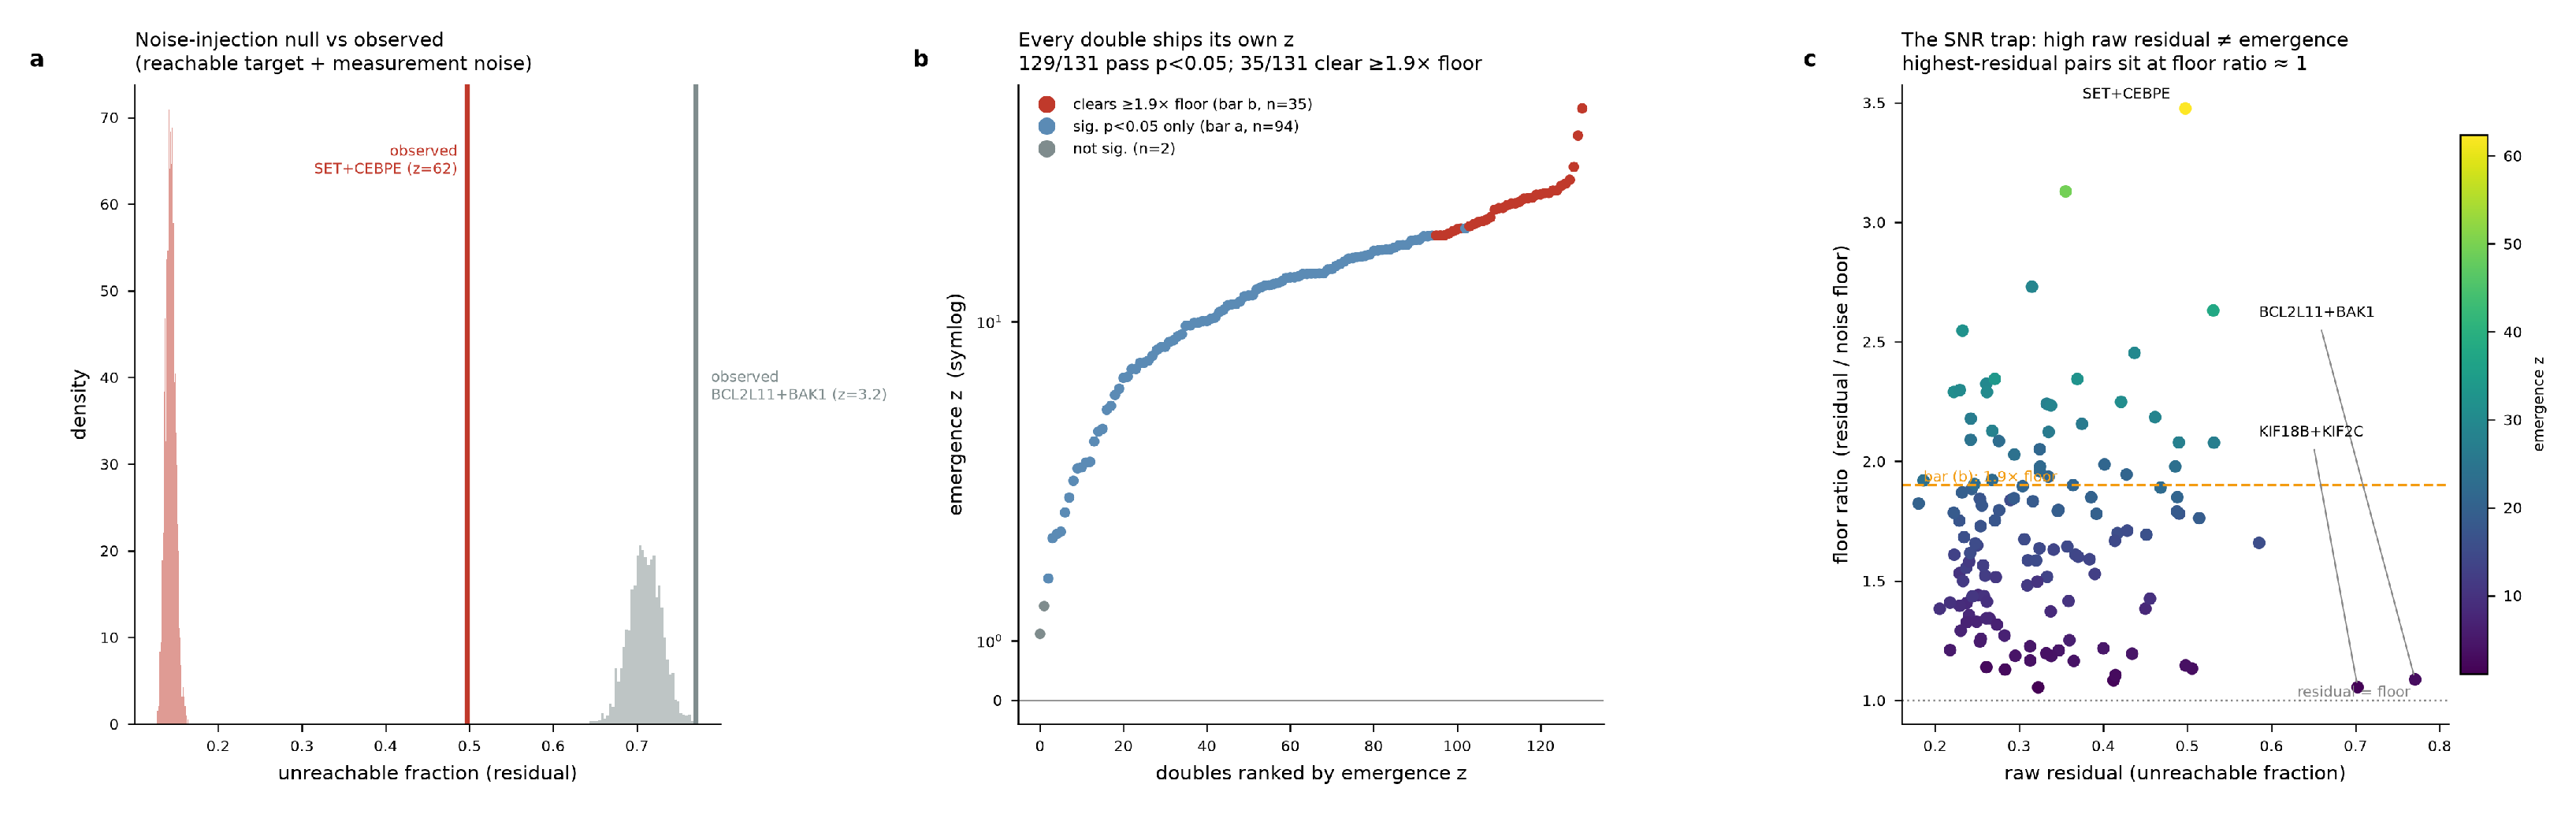
\includegraphics[width=0.92\textwidth]{figS1}
\caption{\textbf{The noise-injection certificate in detail.} For each Norman double, the observed
unreachable fraction is compared against the reachable-target noise null; the bar-(a) significance
call ($p<0.05$, $129/131$) and the stricter bar-(b) floor call ($1.9\times$, $35/131$) are shown,
along with the ``SNR trap'' panel in which low-magnitude pairs show inflated \emph{raw} residuals
but collapse under the noise-aware $z$. This is the per-pair detail behind
Fig.~\ref{fig:certificate}.}
\label{fig:supp-certificate}
\end{figure*}

\begin{figure*}[h]
\centering
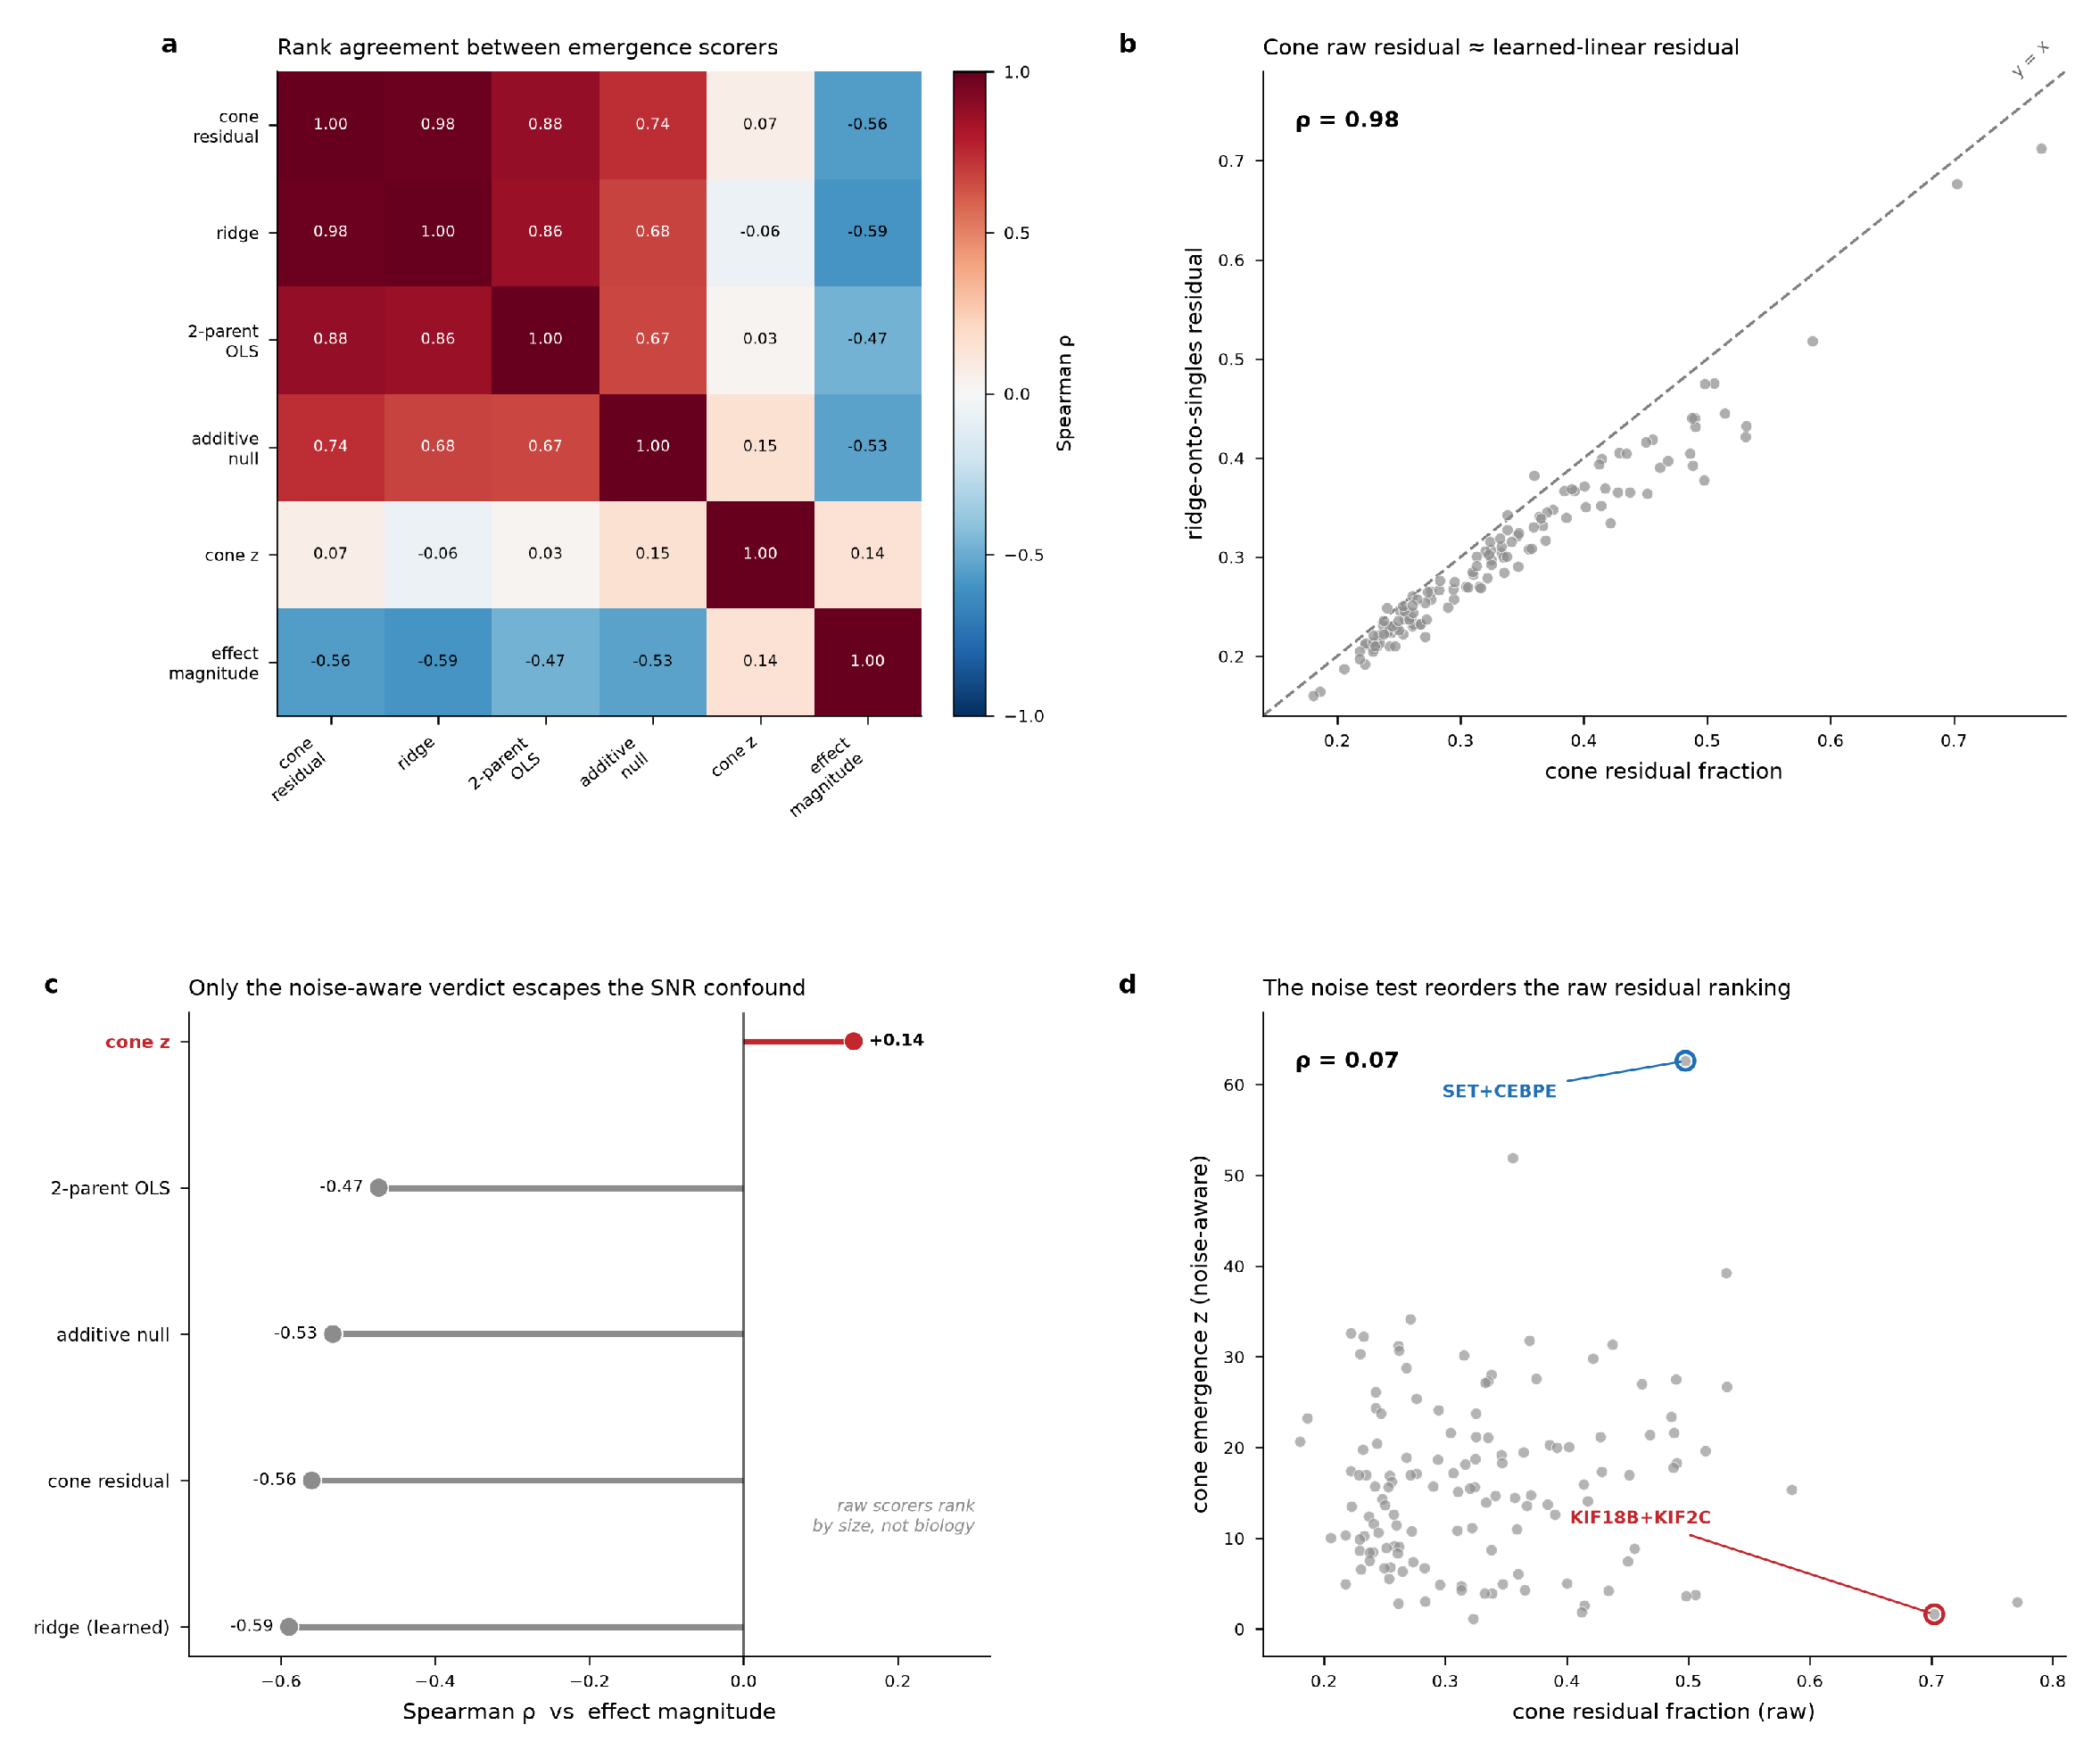
\includegraphics[width=0.92\textwidth]{figS2}
\caption{\textbf{All raw emergence rankers are magnitude-confounded; only the noise-aware $z$
escapes.} The cone residual agrees with a ridge interaction model (Spearman $0.98$), and every raw
ranker---cone residual, non-additivity, ridge and OLS interaction residuals---correlates negatively
with effect magnitude ($-0.47$ to $-0.59$); the noise-aware $z$ is the only score that is
magnitude-free ($+0.14$). This is the confound diagnostic behind the head-to-head of
Fig.~\ref{fig:headtohead}.}
\label{fig:supp-headtohead}
\end{figure*}

\begin{figure*}[h]
\centering
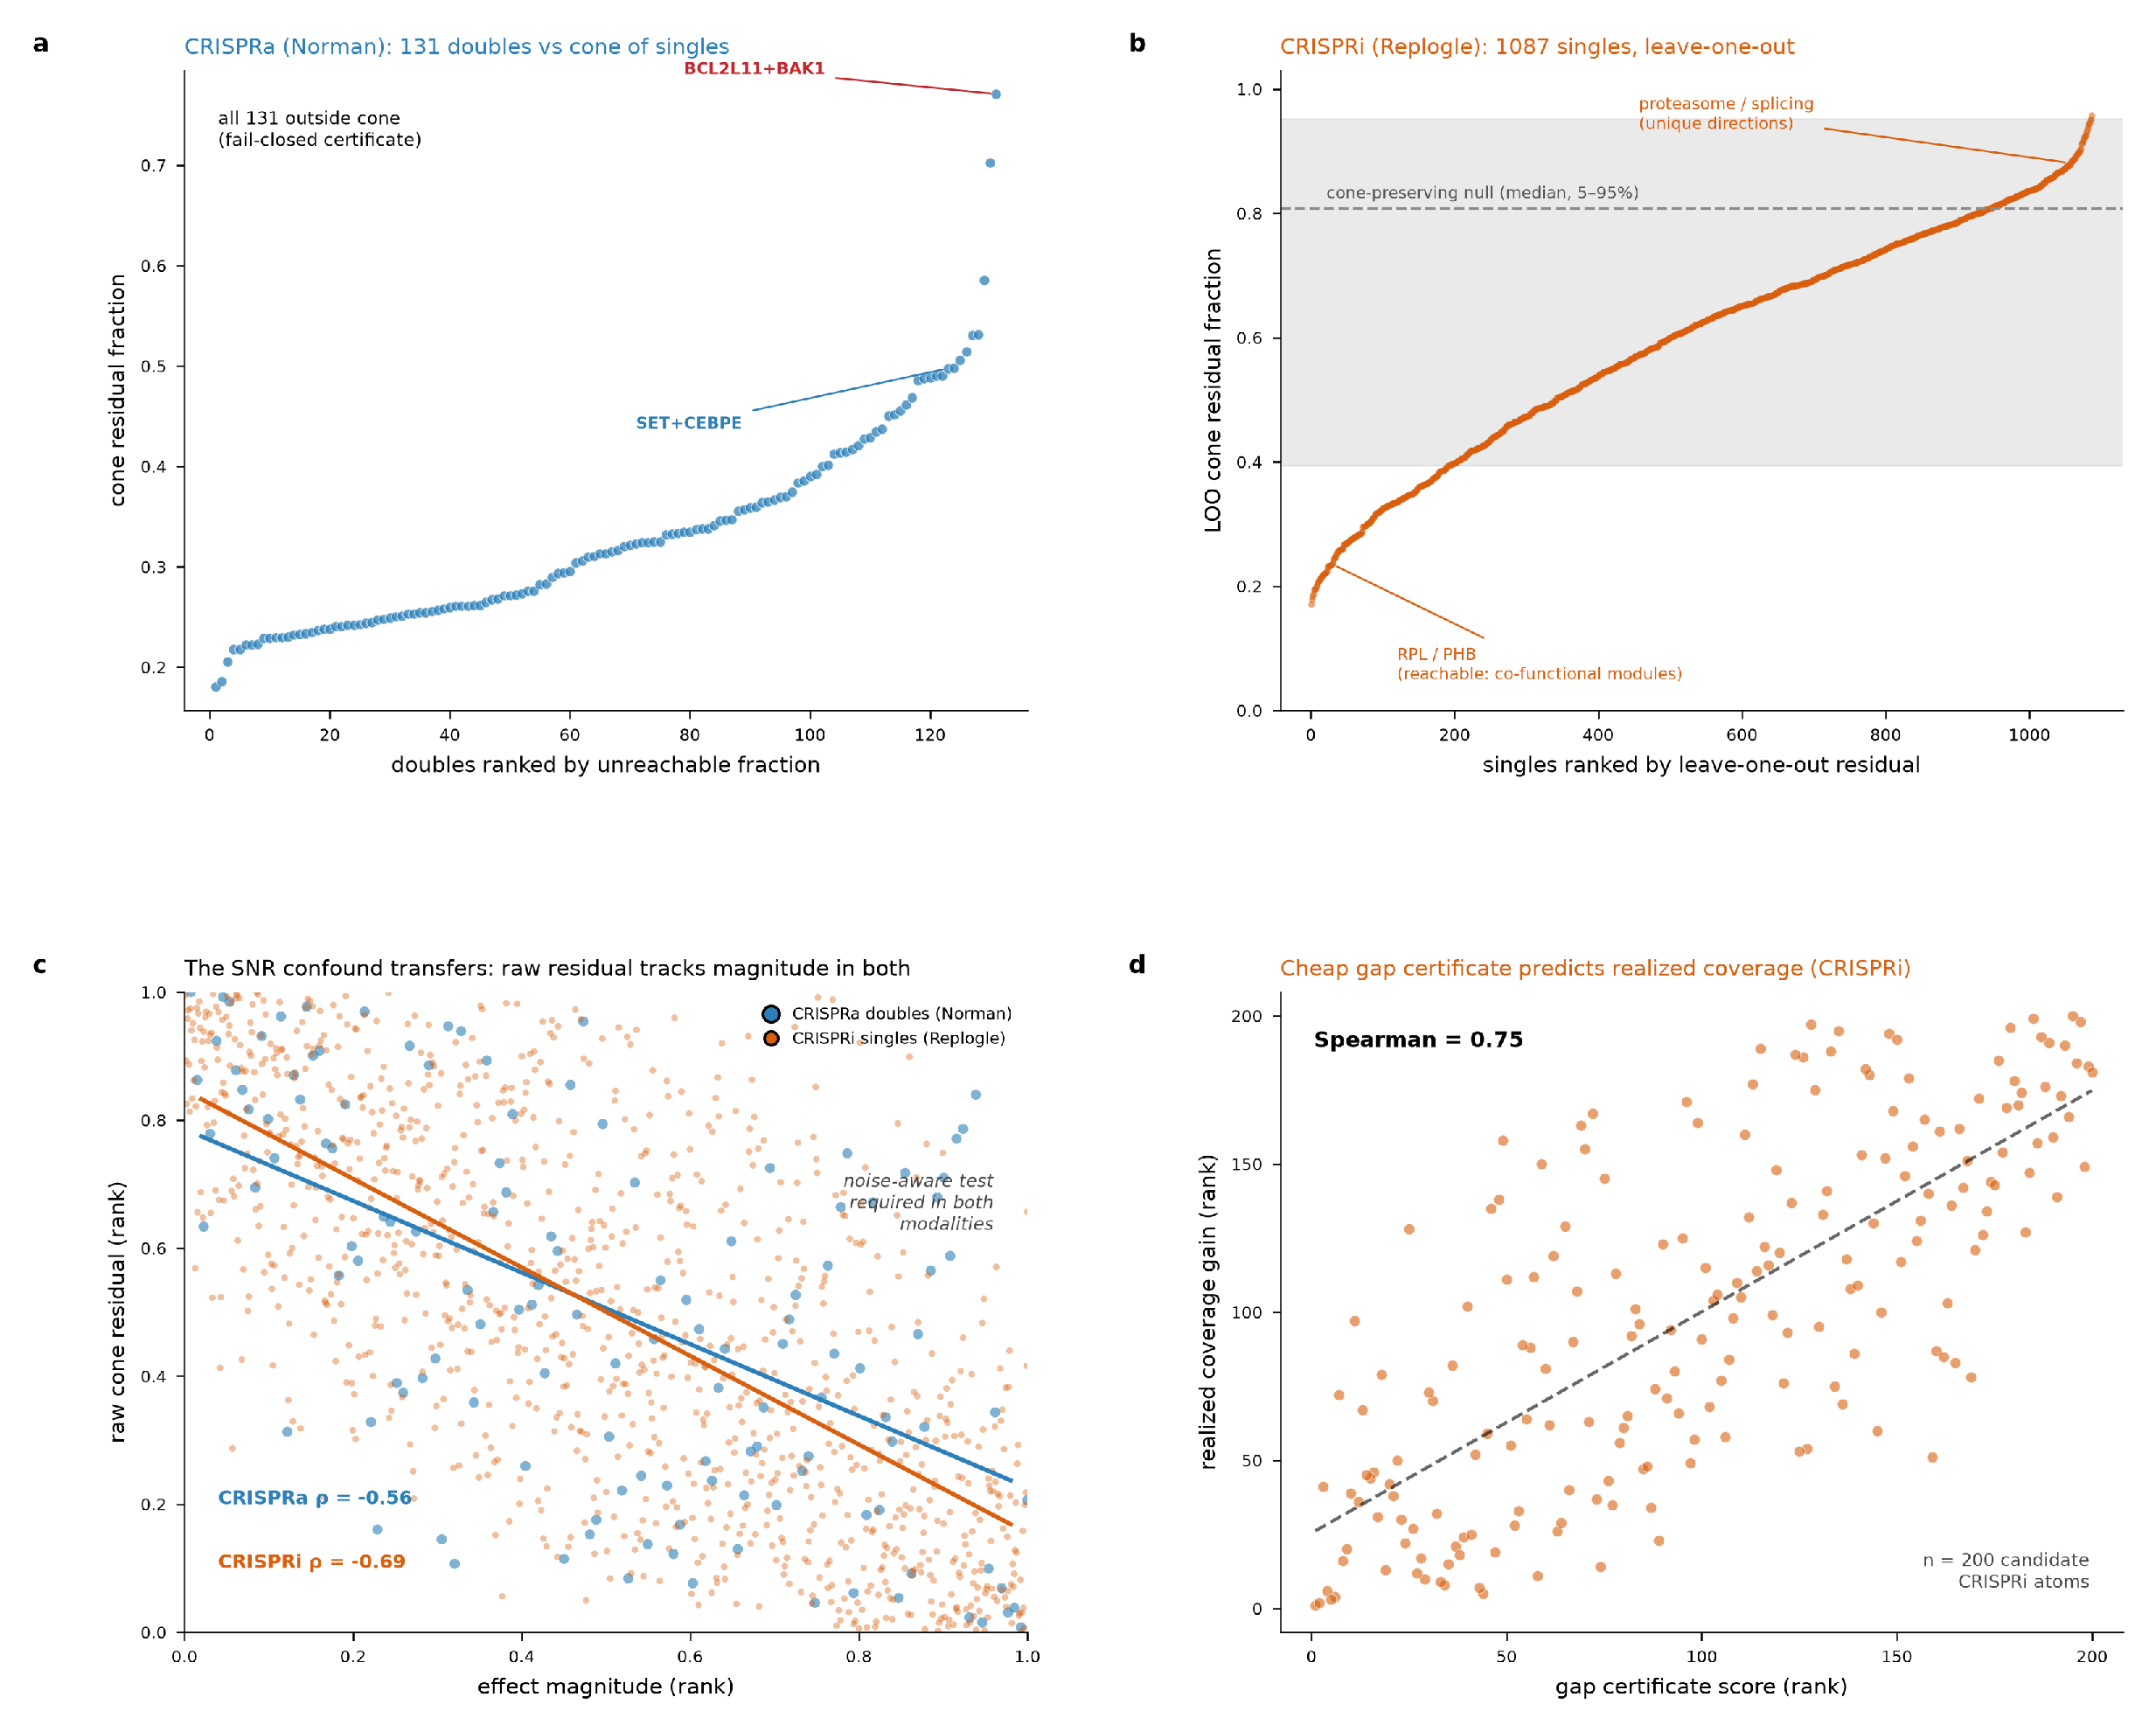
\includegraphics[width=0.92\textwidth]{figS3}
\caption{\textbf{Cross-modality reproduction on Replogle CRISPRi.} The same pipeline run on the
Replogle K562 essential-gene CRISPRi screen reproduces the leave-one-out emergence spectrum and the
certificate-versus-realized agreement (Spearman $0.75$); the SNR/magnitude confound is present in
both CRISPRa ($-0.56$) and CRISPRi ($-0.69$) and is removed by the noise-aware score in both. This
is a geometry-transfer check, distinct from the orthogonal-screen certificate transfer of
Fig.~\ref{fig:crossscreen}, which uses CaRPool-seq.}
\label{fig:supp-crossmodality}
\end{figure*}

\clearpage
\subsection*{Reproducibility}
Every number and figure in this manuscript is produced by a pinned, single-command reproduction
of the released code (\texttt{reachability.py}, \texttt{combicone.py}, \texttt{neural\_baseline.py})
against the published effect matrices of \citet{Norman2019} and \citet{Wessels2023}. The
combinatorial-triage API, its test suite, the $k$-way validation scripts, and a deterministic,
data-free tutorial notebook accompany the code; a canonical facts sheet ties each reported value to
the analysis output that produced it.


\end{document}
